%=============================================================================
% Packages

\NeedsTeXFormat{LaTeX2e} [1994/06/01]
\documentclass [10pt,letterpaper] {article}
\usepackage[reqno,intlimits,sumlimits]{amsmath}
\usepackage{fancyhea}
\usepackage{float}
\usepackage{graphicx}
\usepackage{url}


%\numberwithin{equation}{section}
\renewcommand{\baselinestretch}{1.2}
\renewcommand{\arraystretch}{1}

%-----------------------------------------------------------------------------
%  Define the page layout.

\setlength{\oddsidemargin}{0.0in} \setlength{\hoffset}{0in}
\setlength{\textwidth}{6.5in}

\setlength{\topmargin}{-0.2cm} \setlength{\voffset}{0.0in}
%\setlength{\topmargin}{0cm} \setlength{\voffset}{0.0in}
\setlength{\textheight}{8.5in}

%-----------------------------------------------------------------------------
%  Define the page headers.

\pagestyle{fancy}

\lhead{\it Tim$^{ML}$ 3.4} \chead{} \rhead{\thepage} \lfoot{Mark Bakker} \rfoot{\today}
\cfoot{}

\setlength{\headrulewidth}{0.0pt}
\setlength{\footrulewidth}{0.0pt}
%-----------------------------------------------------------------------------
% Pull in all of the necessary macros.

%=============================================================================
\begin{document}
%=============================================================================
\def\Tim{{\it Tim}$^{\text{ML}}$}
\def\Timsp{{\it Tim}$^{\text{ML}}$ }

\title{{\it Tim}$^{\text{ML}}$\\A Multiaquifer Analytic Element Model\\Version 4.0\\DRAFT}
\author{{\bf Mark Bakker}\\Water Resources Section, Civil Engineering and Geosciences\\
Delft University of Technology, Delft, The Netherlands
\\mark.bakker@tudelft.nl
}
\date{\today}
\maketitle

\begin{figure}[h]
\centering
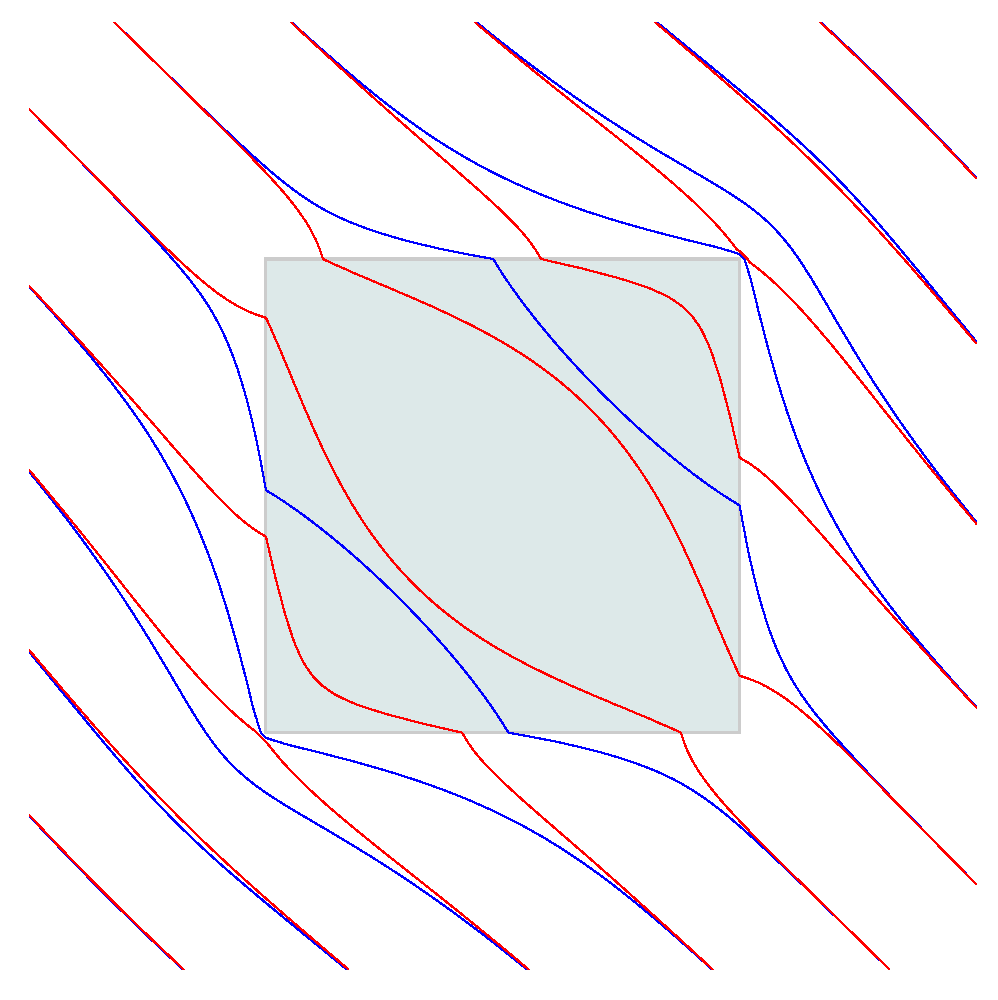
\includegraphics[width=5cm,draft=false]{frontpic.eps}
\end{figure}

\centerline{ARTHUR:
    What manner of man are you that can }
\centerline{\hspace{2cm} summon up   fire without flint or tinder?}
 \centerline{TIM:  I... am an enchanter.}
\centerline{ARTHUR: By what name are you known?} \centerline{TIM:
There are some who call me $\hdots$ Tim.} \centerline{ARTHUR:
Greetings, Tim the Enchanter. } \centerline{\footnotesize Scene
32, Monty Python and the Holy Grail}

\vskip 1cm
\centerline{\copyright Mark Bakker, 2015}
\centerline{\Timsp is free, open--source software and is distributed}
\centerline{under the MIT
License}

\newpage
\tableofcontents

\newpage
\section{Introduction}

\Timsp is a computer program for the simulation of steady-state
multiaquifer flow with analytic elements and consists of a
library of Python scripts and FORTRAN extensions. \Timsp may be applied to an arbitrary number
of aquifers and leaky layers. The head, flow, and leakage between
aquifers may be computed analytically at any point in the aquifer
system. The design of \Timsp is object--oriented and has been kept
simple and flexible. New analytic elements may be added to the
code without making any changes in the existing part of the code.
\Timsp is coded in Python, a free and open-source
programming language; occasional use is made of
FORTRAN extensions to improve performance.

\Timsp includes many multiaquifer analytic
elements including (but not limited to): Constant, Uniform flow, Wells,
Strength--specified linesinks, Head--specified linesinks, Resistance
linesinks, Impermeable walls, Circular areasinks, Polygonal areasinks, Cylindrical
inhomogeneities, Polygonal inhomogeneities, and Embedded multiaquifer domains. Most elements may be located or
screened in multiple layers or aquifers. Utilities have been written for the creation of contour plots and path line plots using the matplotlib package.
Graphical output includes many formats including pdf, eps and png.  Alternatively, grids and layouts may be exported to
Surfer\footnote{Surfer is sold by Golden Software, www.goldensoftware.com} or
MATLAB\footnote{MATLAB is sold by The MathWorks, www.mathworks.com}.
Three-dimensional path lines may be exported into files that can be
imported into the same programs.

\subsection{Approximations}
\Timsp is based on an analytic element formulation for multiaquifer flow with a
number of restrictions. Aquifer parameters and leaky layer parameters must be
piecewise constant. Flow is at steady-state. Unconfined flow in the top aquifer may be approximated by
specifying an average transmissivity. Vertical flux between model layers is computed as the head difference divided by the vertial resistance. Hence, it is assumed that flow remains semi-confined in all layers, except
for in the top layer (i.e., the head in layer $n$ is higher than the top of layer $n$).
The resistance to vertical flow is
neglected within an aquifer, but flow is three--dimensional; the vertical
component of flow in an aquifer is obtained from three--dimensional continuity
of flow. Flow in leaky layers is approximated as vertical.

\subsection{MIT License}

\Timsp is distributed under the MIT License.

Permission is hereby granted, free of charge, to any person obtaining a copy
of \Timsp and associated documentation files (the "Software"), to deal
in the Software without restriction, including without limitation the rights
to use, copy, modify, merge, publish, distribute, sublicense, and/or sell
copies of the Software, and to permit persons to whom the Software is
furnished to do so, subject to the following conditions:

The above copyright notice and this permission notice shall be included in
all copies or substantial portions of the Software.

THE SOFTWARE IS PROVIDED "AS IS", WITHOUT WARRANTY OF ANY KIND, EXPRESS OR
IMPLIED, INCLUDING BUT NOT LIMITED TO THE WARRANTIES OF MERCHANTABILITY,
FITNESS FOR A PARTICULAR PURPOSE AND NONINFRINGEMENT. IN NO EVENT SHALL THE
AUTHORS OR COPYRIGHT HOLDERS BE LIABLE FOR ANY CLAIM, DAMAGES OR OTHER
LIABILITY, WHETHER IN AN ACTION OF CONTRACT, TORT OR OTHERWISE, ARISING FROM,
OUT OF OR IN CONNECTION WITH THE SOFTWARE OR THE USE OR OTHER DEALINGS IN
THE SOFTWARE.

\subsection{Introduction for MLAEM users}
MLAEM\footnote{MLAEM is sold by Strack Consulting, www.strackconsulting.com} is
currently the only other available multiaquifer analytic element model. The
main difference between \Timsp and MLAEM is that in \Timsp leakage between aquifers
is simulated automatically and exactly without the need for specifying
area-elements for leakage. One practical difference is that \Timsp allows for
the specification of one reference point in one aquifer only, while MLAEM
requires the specification of one reference point in every aquifer.

\subsection{Introduction for MATLAB users} There are a lot of similarities
between Python and MATLAB. Both may be run from a command prompt and are
interactive. Three major differences are important when running \Tim. (1) The
object--oriented programming capabilities of Python are much larger and more
elegant than MATLAB. As a practical consequence, a Python method that has been
stored in a file can only be called if the file is first imported (MATLAB often
calls methods by looking up file names). (2) Variables are not automatically matrices in Python. The
numpy package offers the ability to define matrices (called arrays). Array
multiplication is by default term by term. Commands are often similar or identical to
corresponding commands in MATLAB. For example, the function eig(A)
returns the eigenvalues of A. (3) Python is free and open--source.
For more details on the differences between numpy and MATLAB, see http://www.scipy.org/NumPy$\_$for$\_$Matlab$\_$Users.


\subsection{Introduction for MODFLOW users} A comprehensive introduction into
multiaquifer modeling with analytic elements (and especially \Tim) for MODFLOW
users is planned here. For now it is limited to explaining the relationship
between the resistance $c$ of an aquitard (used in \Tim) and the variable
Vcont used in MODFLOW models. The resistance $c$ is the reciprocal of Vcont:
$c=1/\text{Vcont}$.

\subsection{Differences with Version 3 and before}
\Timsp version 4 is not compatible with previous versions. The most important changes are:
\begin{itemize}
\item \Timsp is now imported as {\tt timml} (so no more capitals).
\item The {\tt Model} class does not take the number of aquifer as input anymore. The number of aquifers is determined by \Timsp from the length of the {\tt zb} array.
\item All layer numbering starts at zero at the top layer.
\end{itemize}

\subsection{Release History} \begin{description}
\item Version 0.1. January,
2002. First beta release.
\item Version 1.0. May, 2002. First full release
\item Version 1.1. January 2003. Improvement of speed of aquifer system
inhomogeneities (they are now 5-10 times faster), conversion to Python 2.2,
and inclusion of a large number of hooks, including an experimental iterative
solver, to prepare for inclusion of circular and elliptical inclusions in
future versions.
\item Version 1.2. July 2003. Added Uflow element, resistance
line-sinks, and Model3D command. Fixed inaccuracy with circular area-sinks
regarding large radii. Build in more hooks for version 2 release.
\item
Version 2.0. January 2004. Added ditches, polygonal area-sinks, cylindrical
inhomogeneities, the possibility to model semi-confined aquifer systems, and
three-dimensional path line tracing.
\item Version 2.1. August 2004. Improved
speed, improved accuracy and efficiency of tracing algorithm, improved aquifer
system inhomogeneities; not yet operational for semi-confined flow.
\item
Version 2.1.1. January 2005. Bug fix for resistance line-sinks.
\item Version
3.0.alpha1. February 2006. Addition of polygonal inhomogeneities with the same
number of aquifers inside and outside. Semi-confined flow has been disabled as
it will be replaced by an entirely new formulation before the full 3.0
release. Aquifer system inhomogeneities may be added with the
AquiferSystemInhomogeneity command; the old MakeInhomogeneity command will be
phased out.
\item Version 3.0. February 2007. Switch to numpy and Python 2.4. Semi-confined
flow option permanently removed; a better replacement is in the works. Number
of fixes in trace routine. New webpage. Accuracy improvements FORTRAN extension.
FORTRAN extension compiled with GNU compiler.
\item Version 3.1. July 2007. Percolating resistance line-sinks and some bug fixes.
\item Version 3.2. August 2008. Impermeable walls and some bug fixes. Simultaneous release of versions for Python 2.4 and 2.5.
\item Version 3.3.alpha. October 2008. Replaced MakeInhomSide by MakeInhomPolySide. Automatically checks for aqin and aqout. PolyInhomData checks for clockwise or counter-clockwise. New element Lake, including partially percolating bottom; needs installation of matplotlib and shapely. Interactive plotting with timcontour; needs installation of matplotlib.
\item Version 3.3. May 2009. The new Lake element had been tested and works well with all elements. Restriction is still that the entire outside of the lake needs to be the background aquifer. This restriction will be removed in the next release.
\item Version 3.4. March 2010. Added interactive graphical output using the matplotlib package. Updated the manual to use IPython as the preferred Python shell. Updated the new installation requirements.
\item Version 4.0.alpha. April 2015. Layers numbering starts at zero.
\end{description}

\subsection{Acknowledgement}
Development of \Timsp was funded in part by:
\begin{itemize}
\item Intera, Inc., Austin, TxX
\item  Ecosystems
Research Division, United States
Environmental Protection Agency, Athens, GA
\item WHPA, Bloomington, IN, a Layne Christensen company.
\item Amsterdam Water Supply, Brabant Water, Waterbedrijf Limburg, in
collaboration with Artesia.
\item United States Bureau of Reclamation.
\end{itemize}
Dr. Stephen Kraemer of USEPA assisted in
beta--testing and comparisons with MODFLOW.
\\Dr. Vic Kelson of WHPA co-developed the original design and has been providing feedback during
the entire development process of \Tim.
\\Dr. Philippe LeGrand contributed the script for generating windows
installers.
\\Frans Schaars of Artesia extensively tested the trace routine through application to practical problems.
\subsection{Plans}

There is a long list of plans for the expansion of \Tim.
Implementation of the
different ideas depends on available time, funds, and
inspiration. If you want to contribute to the development
of \Tim, either through code development or through
financial support, please contact Mark Bakker at
markbak@gmail.com. Several of the listed elements are
already in some stage of development. Plans for \Timsp include:
\begin{itemize}
\item Lakes that can be connected or (partially) inside inhomogeneities.
\item Leaky walls and leaky faults.
\item Elliptical inhomogeneities with an arbitrary
number of aquifers and leaky layers both inside and outside the
inhomogeneity. They have been developed and implemented fully but have not been
released as they require an additional Python extension in C++, which cannot be pickled. When interested,
email the developer.
\item Local percolating conditions (now only along ResLineSinks and Lakes).
\item Nested inhomogeneities (one inhomogeneity or lake inside another inhomogeneity).
\item Improvement of computational speed.
\item Improvement of accuracy of short high-order elements.
\item Better interfacing with existing GUIs and possible linkage with an existing open--source GUI.
\item Addition of utilities to do
contaminant transport.
\item GUI for postprocessing using Matplotlib (prototype done in Tkinter).
\end{itemize}

\subsection{\Timsp website}
\Timsp code is hosted on \url{github}

\newpage
\section{Installation}
The following free, open-source software is required to run \Tim:
Python version 2.X, the packages numpy, scipy, and matplotlib. The shapely package is needed for the use of Lake elements (optional). \Timsp uses a FORTRAN extension which means that \Timsp is unfortunately both platform dependent
and Python version dependent. 

Although it is possible to download all required Python packages separately, it is much easier to install one of the Python installers that comes with a large selection of popular packages. Three main options are Anaconda, Enthought, and PythonXY. This manual is written for Anaconda users. Use of the other distributions only differs in how IPython is started.


\newpage

\section{Application}
It may be beneficial (actually it is highly recommended) to spend some time
going through an introductory Python tutorial if you are not familiar with
Python; many free tutorials are available from the Python website. An introduction to Python for Exploratory computing can be found at: \url{http://mbakker7.github.io/exploratory_computing_with_python/}

Application
of \Timsp requires a certain intelligence from the user. Very few assertions
are implemented in the code to verify that valid input variables are entered.
(The only ones that are checked correspond to errors that the developer kept
making or requests from users.) When \Timsp returns an error, read the error carefully. If the last
line of the error message starts with something like {\tt AssertionError: TimML Input error:}
then this is an assertion error indicating you are trying to enter invalid
data and instructions are given on what you should do.

\subsection{Starting a model}
In this manual, \Timsp is run from the IPython prompt. Start the Anaconda Launcher and launch the IPython-Qtconsole. 
At the Python command prompt, import {\tt timml} (`{\tt In []:}' is used for the Python prompt in this manual; IPython adds a input number between the square brackets):
\\{\tt In []: from timml import *}
\\It may take a couple of seconds to load everything. If you
have not installed \Timsp correctly, you will get the following error message:
\begin{verbatim}
In []: from timml import *
---------------------------------------------------------------------------
ImportError                               Traceback (most recent call last)
<ipython-input-2-9b20be32f415> in <module>()
----> 1 from timml import *

ImportError: No module named timml
\end{verbatim}
When you create an input file, the line {\tt from timml import *} must be the
first line of your file. The next command must be the creation of a model,
which must be given a name, for example {\tt ml}. All elements will be added to this model.
\begin{itemize}
\item[{\tt In []:}] {\tt ml = Model(k,zb,zt,c,n=[],nll=[])} where
    \begin{itemize}
    \item {\tt k} is a list\footnote{A list is a sequence separated by commas and between square brackets,
    such as: [1,2,3]} of permeabilities of the aquifers starting
    from the top down.
    \item {\tt zb} is a list of bottom elevations of the aquifers
    from the top down (Note: this may be counter intuitive, so be
    careful.) The number of aquifers {\tt Naquifers} is determined from the length of {\tt zb}.
    \item {\tt zt} is a list of top elevations of the aquifers
    from the top down
    \item {\tt c} is a list of resistances (dimension: time) of separating layers
    between aquifers. The list starts with the bottom of aquifer 1 and is thus
    {\tt Naquifers}$-1$ long.
    \item {\tt n} is a list with the porosities of the aquifers. If it is not entered, it is set to 0.3.
    \item {\tt nll} is a list with the porosities of the leaky layers. If it is not entered, it is set to 0.3.
%    \item {\tt type} is either {\tt 'conf'} (default) which means the aquifer
%    system is confined, or {\tt 'semi'} which means the aquifer is semi-confined, with
%    a leaky layer and fixed water table on top of the aquifer system.
%    \item {\tt hstar} is the head on top of the leaky layer in case the type is {\tt semi} (otherwise
%    it does not have to be specified).
    \end{itemize}
\end{itemize}
Note that aquifers are numbered from the top down in \Tim, starting with number
0. Also note that any parameters in the argument list that are followed by an equal sign
(such as {\tt n=[]}) are optional parameters.
\\Alternatively, when 3D flow is modeled, a model may be constructed with the
command
\begin{itemize}
\item[{\tt In []:}] {\tt ml = Model3D(z=[1,0.5,0],kh=1.0,kzoverkh=1.0)} where
    \begin{itemize}
    \item {\tt z} is a list with the top elevations of all the layers (from the top down) that an aquifer is divided
    into; the last value is the bottom of the aquifer.
    \item {\tt kh} is the horizontal hydraulic conductivity of the aquifer and may either be one value or a list/tuple/array with a value for each layer.
    \item {\tt kzoverkh} is the vertical anisotropy ratio $k_z/k_h$ and may either be one value or a list/tuple/array with a value for each layer.
    \end{itemize}
\end{itemize}


\subsection{Adding analytic elements}
The following elements may be added to the model:
\begin{itemize}
\item[{\tt In []:}] {\tt Constant(modelParent,xr,yr,head,layer,label=None)} where
    \begin{itemize}
     \item {\tt modelParent} is the model to which the element is
    added
    \item {\tt xr,yr} is the location of the reference point
    \item {\tt head} is the head at the reference point
    \item {\tt layer} is the number of the aquifer in which the reference point is applied
    \item {\tt label} is an optional character string representing the label of the element
    (if you want to access this element later, it may be hard if you don't give it a label)
    \end{itemize}
    Only one {\tt Constant} element may be added to a model\footnote{This is different than in MLAEM, where
    a constant must be specified for every layer.}. It is not
    checked in \Timsp whether more than one {\tt Constant} is
    added to the model\footnote{This is one of those places where the
    intelligence of the user is expected.}.
\item[{\tt In []:}] {\tt Uflow(modelParent,grad,angle,label=None)} where
    \begin{itemize}
     \item {\tt modelParent} is the model to which the element is
    added
    \item {\tt grad} is the gradient of the head (positive)
    \item {\tt angle} is the direction of uniform flow, in degrees measured counter-clockwise with respect to positive
    $x$ (East).
    \item {\tt label} is an optional character string representing the label of the element.
    \end{itemize}
\item[{\tt In []:}] {\tt Well(modelParent,xw,yw,Qw,rw,layers,label=None)} where
    \begin{itemize}
    \item {\tt modelParent} is the model to which the element is
    added
    \item {\tt xw,yw} is the location of the well
    \item {\tt Qw} is the discharge [L$^3$/T] of the well (positive for
    taking water out)
    \item {\tt rw} is the radius of the well
    \item {\tt layers} is the number of the model layer in which the well is screened or a list of layer numbers when the well is screened in multiple layers. 
    \item {\tt label} is an optional character string representing the label of the element.
    \end{itemize}
    When the well is screened in more than one layer (a multi--aquifer well), the
    discharge of the well is divided over the aquifers such that
    the heads in the aquifers are equal.
\item[{\tt In []:}] {\tt LineSink(modelParent,x1,y1,x2,y2,sigma,layers,label=None)} where
    \begin{itemize}
    \item {\tt modelParent} is the model to which the element is
    added
    \item {\tt x1,y1,x2,y2} are the left and right end points of
    the line-sink
    \item {\tt sigma} is the strength [L$^2$/T] of the line-sink per unit length
    of line-sink (positive for taking water out); the strength is constant
    along the element.
    \item {\tt layers} is the number of the model layer in which the line-sink is screened or a list of layer numbers when the line-sink is screened in multiple layers. 
    \item {\tt label} is an optional character string representing the label of the element.
    \end{itemize}
    When the line-sink is screened in more than one aquifer, the
    strength of the line-sink is divided over the aquifers such that
    the heads in the aquifers are equal. Note that if the strength is zero, this means that
    you are modeling a highly conductive, vertical fault zone.
\item[{\tt In []:}] {\tt HeadLineSink(modelParent,x1,y1,x2,y2,head,layers,label=None)}
    \begin{itemize}
    \item {\tt modelParent} is the model to which the element is
    added
    \item {\tt x1,y1,x2,y2} are the left and right end points of
    the line-sink
    \item {\tt head} is the head at the center of the line-sink
    \item {\tt layers} is the number of the model layer in which the line-sink is screened or a list of layer numbers when the line-sink is screened in multiple layers. 
    \item {\tt label} is an optional character string representing the label of the element.
    \end{itemize}
\item[{\tt In []:}] {\tt ResLineSink(modelParent,x1,y1,x2,y2,head,res,width,layers=[1],label=None,bottomelev=None)}
    \begin{itemize}
    \item {\tt modelParent} is the model to which the element is
    added
    \item {\tt x1,y1,x2,y2} are the left and right end points of
    the line-sink
    \item {\tt head} is the head at the center of the line-sink
    \item {\tt res} is the resistance of the bottom of the line-sink against in/outflow.
    \item {\tt width} is the width of the line-sink
    \item {\tt layers} is the number of the model layer in which the line-sink is screened or a list of layer numbers when the line-sink is screened in multiple layers. 
    \item {\tt label} is an optional character string representing the label of the element.
    \item {\tt bottomelev} is the elevation of the bottom of the (leaky) resistance layer at the bottom of the line-sink.
    This value is only used to check whether there is a hydraulic connection between the computed head and the bottom
    of the leaky layer. When such conditions may occur, the solution needs to be computed iteratively using the
    command {\tt ml.solve(doIterations=True)}.
    \end{itemize}
\item[{\tt In []:}] {\tt LineSinkDitch(modelParent,xylist,Q,res,width,layers=[1],label=None)}
    \begin{itemize}
    \item {\tt modelParent} is the model to which the element is
    added
    \item {\tt xylist} is a list of $(x,y)$ pairs of the nodes of
    the line-sink ditch, such as
    [(0,0),(10,0),(10,10),(0,10)].
    \item {\tt Q} is the total discharge [L$^3$/T] of the ditch. The head in
    the ditch will be constant, but is {\it a priori} unknown.
    \item {\tt res} is the resistance of the ditch against in/outflow.
    \item {\tt width} is the width of the ditch
    \item {\tt layers} is the number of the layer in which the ditch is
    screened.
    \item {\tt label} is an optional character string representing the label of the element.
    \end{itemize}
\item[{\tt In []:}] {\tt LineDoubletImp(modelParent,x1,y1,x2,y2,order=0,layers=[1],label=None)}
    \begin{itemize}
    \item {\tt modelParent} is the model to which the element is
    added
    \item {\tt x1,y1,x2,y2} are the left and right end points of
    the section of impermeable wall.
    \item {\tt order} is the order of the solution. The no-flow condition is applied at order+1 points
    along the wall segment. \emph{Order cannot be higher than 8} for the current implementation. Note: these elements
    are not magic. To obtain an accurate solution it may be necessary to discretize the wall in multiple sections.
    \item {\tt layers} is the number of the model layer in which the impermeable wall is screened or a list of layer numbers when the impermeable wall is screened in multiple layers. 
    \item {\tt label} is an optional character string representing the label of the element.
    \end{itemize}
\item[{\tt In []:}] {\tt CircAreaSink(modelParent,xp,yp,Rp,infil,layer,label=None)} where
    \begin{itemize}
    \item {\tt modelParent} is the model to which the element is
    added
    \item {\tt xp,yp} is the center of the circular area-sink
    \item {\tt Rp} is the radius of the area-sink
    \item {\tt infil} is the areal infiltration rate [L/T] of the
    area-sink (positive for putting water into the aquifer)
    \item {\tt layer} is the number of the model layer to which 
    the area-sink is added.
    \item {\tt label} is an optional character string representing the label of the element.
    \end{itemize}
\item[{\tt In []:}] {\tt PolyAreaSink(modelParent,xylist,infil,label=None)} where
    \begin{itemize}
    \item {\tt modelParent} is the model to which the element is
    added
    \item {\tt xylist} is a list of $(x,y)$ pairs of the nodes of
    the area-sink boundary given in counter clockwise
    direction (this is not checked by the model!), such as
    [(0,0),(10,0),(10,10),(0,10)]; the model will close the
    polygon automatically (so don't give the begin node again at
    the end)
    \item {\tt infil} is the areal infiltration rate [L/T] of the
    area-sink (positive for putting water into the aquifer). The infiltration
    rate is constant over the area-sink.
    \item {\tt label} is an optional character string representing the label of the element.
    \end{itemize}
    A polygonal area-sink is automatically added to layer 0. The sides of a polygonal area-sink are exact (and hence, the lengths of the segments that make up the boundary don't effect the accuracy of the solution as they do for PolygonInhom or Lake elements, for example).
\end{itemize}

\begin{itemize}
\item[{\tt In []:}] {\tt Lake(ml,xylist,hlake,cbot,Hbot,nbot=0.3,Lmax=None,areatol=0.2)} where
    \begin{itemize}
     \item {\bf Lake} elements are currently not included in TimML
    \item {\tt ml} is the model to which the lake is added
    \item {\tt xylist} is a list of $(x,y)$ pairs of the corners of the polygon that bounds the lake. The first point
    does not have to be repeated to close the polygon; it is closed automatically.
    \item {\tt hlake} is the uniform water level in the lake.
    \item {\tt cbot} is the resistance of the bottom of the lake
    \item {\tt Hbot} is the thickness of the bottom of the lake, i.e., the vertical hydraulic conductivity of the lake sediment is Hbot/cbot.
    \item {\tt nbot} is the porosity of the lake bottom; it is set to 0.3 by default.
    \item {\tt Lmax} is the maximum length of a side. When it is not None, the provided list of $(x,y)$ values
    is expanded such that each segment of the boundary is at most {\tt Lmax} long.
    \item {\tt areatol} is the tolerance used to determine whether convergence is achieved when iterating for the size of the percolating area. The default value is 0.2 and it rarely if ever needs to be smaller.
    \end{itemize}
    Lakes have a fixed and uniform water level, a resistance at the bottom, and are bounded by a polygon. Lakes are added automatically to model layer 0. 
Lakes are modeled using the approach described in Bakker (2007). Lakes may not share boundaries with other lakes and may not be inside or overlap inhomogeneities. The boundary of the lake is made-up of second-order line elements. Boundary segments must be made sufficiently short to obtain an accurate solution. The accuracy of the solution may be verified visually: both the head contours must be continuous across the boundary and the tangent to the head contours must be continuous across the boundary (since the aquifer properties don't change from outside the lake to below the lake). An example of an inaccurate solution is given in the Examples section, so you know what to look for. 
\end{itemize}

\subsection{Inhomogeneous aquifer properties}
Three kinds of inhomogeneities may be added: polygonal inhomogeneities, cylindrical inhomogeneities,
and aquifer system inhomogeneities.

\subsubsection{Multi-aquifer polygonal inhomogeneities}
Multi-aquifer polygonal inhomogeneities need to have the same number of
aquifers inside and outside the polygon. Model layer 0 on the inside is connected
to model layer 0 on the outside, etc. Properties of all aquifers and leaky layers may
differ between the inside or the outside, but they don't have to: if you want to change
only the transmissivity of aquifer 2 and leave the rest the same, that is fine too, but
the modeling process will be the same. Inhomogeneities may share boundaries. Inhomogeneities may be nested
inside other inhomogeneities, but they can only be modeled if you enter the smaller inhomogeneity \emph{before} the larger inhomogeneity. 

When modeling an inhomogeneity,
aquifer data for each inhomogeneity must be entered first:
\begin{itemize}
\item[{\tt In []:}] {\tt PolygonInhom(modelParent,Naquifers,k,zb,zt,c,xylist,n=[],nll=[])} where
    \begin{itemize}
    \item {\tt modelParent} is the model to which the aquifer data is
    added
    \item {\tt k} is a list of permeabilities of the aquifers starting
    from the top down.
    \item {\tt zb} is a list of bottom elevations of the aquifers
    from the top down (Note: this may be counter intuitive, so be
    careful.)
    \item {\tt zt} is a list of top elevations of the aquifers
    from the top down
    \item {\tt c} is a list of resistances (dimension: time) of separating layers
    between aquifers, starting with the bottom of aquifer 0. Hence, the
    length of this list is {\tt Naquifers}$-1$.
    \item {\tt xylist} is a list of $(x,y)$ pairs of the nodes of
    the inhomogeneity boundary (can be either clockwise or counter clockwise); the model will close the
    polygon automatically (so don't give the begin node again at
    the end)
    \item {\tt n} is a list with the porosities of the aquifers. If it is not entered, it is set to 0.3.
    \item {\tt nll} is a list with the porosities of the leaky layers. If it is not entered, it is set to 0.3.
    \end{itemize}
\end{itemize}
Sides of an inhomogeneity are added as polylines. Each polyline must have one
     aquifer system on the left side and one aquifer system on the right side. Line-elements that
are put along the polyline will have the same order. When the aquifer on one of
the sides changes, or you want a different order of the line elements, you must
start a new inhomogeneity side. The command for adding elements along an
inhomogeneity side is
\begin{itemize}
\item[{\tt In []:}] {\tt
MakeInhomPolySide(ml,xylist,order,closed=False):} where
    \begin{itemize}
    \item {\tt modelParent} is the model to which the element is
    added
    \item {\tt xylist} is a list of $(x,y)$ pairs of the nodes of
    the polyline that is the (part of the) boundary of an inhomogeneity. 
    The aquifer on the left side of the polyline (going from point 1 to 2 to 3 etc.) must
    be the same for all segments of the polyline. Similarly, the aquifer on the right side of the polyline (going from point 1 to 2 to 3 etc.) must
    be the same for all segments of the polyline.
    This boundary must coincide with the boundary of
    an inhomogeneity specified with PolygonInhom, although it may have more nodes along each
    side, i.e., one straight segment of PolygonInhom may be subdivided into
    multiple segments with MakeInhomPolySide, as long as they all lie on the same
    straight line.
    \item {\tt order} is the order of the line elements that are put along the
    polyline. Maximum order is 8.
    \item {\tt closed} is a flag that is {\tt False} by default. When it is
    {\tt True} (or 1), the polyline will be closed (so don't repeat the first
    point of the polyline again, just set the {\tt closed} to {\tt True}
    \end{itemize}
\end{itemize}
It is essential that sides are added along the entire inhomogeneity boundary. When inhomogeneities share boundaries, don't repeat the shared
boundary.
Note that this function replaces the deprecated \texttt{MakeInhomSide}, which was included in versions prior to 3.3. It  worked the same
except that the aquifers on the left and right sides had to be provided as arguments\footnote{This lead to too many input errors, so it is
now figured out by TimML}.

\subsubsection{Cylindrical inhomogeneities}
Cylindrical inhomogeneities intersect all aquifers. the number of aquifers and leaky layers
must be the same inside and outside the cylinder. Both the transmissivity of the aquifers and the resistance of leaky
layers may be different between the inside and the outside of the cylinders.  \emph{May} is the operative word here as they
don't have to be different (just like for polygonal inhomogeneities). For example to model a sandy hole in a leaky clay layer
you can change the resistance of one leaky layer only and leave all other resistances and transmissivities
the same. To enter a cylindrical inhomogeneity, you have to define the aquifer data
on the inside of the cylinder first

\begin{itemize}
\item[{\tt In []:}] {\tt inhom1 = CircleInhomData(modelParent,k,zb,zt,c,xc,yc,R,n=[],nll=[])} where
    \begin{itemize}
    \item {\tt modelParent} is the model to which the aquifer data is
    added
    \item {\tt k} is a list of permeabilities of the aquifers starting
    from the top down.
    \item {\tt zb} is a list of bottom elevations of the aquifers
    from the top down (Note: this may be counter intuitive, so be
    careful.)
    \item {\tt zt} is a list of top elevations of the aquifers
    from the top down
    \item {\tt c} is a list of resistances (dimension: time) of separating layers
    between aquifers, starting with the bottom of aquifer 1. Hence, the
    length of this list is {\tt Naquifers}$-1$.
    \item {\tt xc,yc} is the center of the cylinder
    \item {\tt R} is the radius of the cylinder
    \item {\tt n} is a list with the porosities of the aquifers. If it is not entered, it is set to 0.3.
    \item {\tt nll} is a list with the porosities of the leaky layers. If it is not entered, it is set to 0.3.
    \end{itemize}
    CircleInhomData should be given a name ({\tt inhom1} in the input line above) so that it can be used to
    define the inside of an inhomogeneity.

\end{itemize}
Then a cylindrical inhomogeneity may be added:
\begin{itemize}
\item[{\tt In []:}] {\tt
CircleInhom(modelParent,order,aqin,aqout,label=None)} where
    \begin{itemize}
    \item {\tt modelParent} is the model to which the element is
    added
    \item {\tt order} is the number of terms that is used in the
    series expansion (the more the more accurate and the slower the solution).
    \item {\tt aqin} is the {\tt CircleInhomData} on the inside of the
    inhomogeneity (that would be {\tt inhom1} in the example
    above).
    \item {\tt aqout} is the aquifer data on the outside of the
    inhomogeneity. This is the background aquifer data defined
    with {\tt Model}. For example, if the model is called {\tt ml}
    then the aquifer data on the outside is {\tt ml.aq} ({\tt aq}
    is an attribute of {\tt Model}).
    \item {\tt label} is an optional character string representing the label of the element.
    \end{itemize}
\end{itemize}
Warning: cylindrical inhomogeneities may become inaccurate when the radius is very large
compared to the leakage factor. This can be fixed, but has not been
implemented.

\subsubsection{Aquifer system inhomogeneities}
{\bf Aquifer system inhomogeneities} are not included in the current version of TimML.
Aquifer system inhomogeneities have either \emph{one} aquifer
outside (defined with {\tt Model}) and an arbitrary number of aquifers and
leaky layers inside or vice versa. Aquifer system inhomogeneities may
not share boundaries. To enter an aquifer system inhomogeneity, first enter aquifer data for the inhomogeneity:
\begin{itemize}
\item[{\tt In []:}] {\tt inhom1 = PolygonInhom(modelParent,Naquifers,k,zb,zt,c,xylist,n=[],nll=[])} where
    \begin{itemize}
    \item {\tt modelParent} is the model to which the aquifer data is
    added
    \item {\tt Naquifers} is the number of aquifers
    \item {\tt k} is a list of permeabilities of the aquifers starting
    from the top down.
    \item {\tt zb} is a list of bottom elevations of the aquifers
    from the top down (Note: this may be counter intuitive, so be
    careful.)
    \item {\tt zt} is a list of top elevations of the aquifers
    from the top down
    \item {\tt c} is a list of resistances (dimension: time) of separating layers
    between aquifers, starting with the bottom of aquifer 1. Hence, the
    length of this list is {\tt Naquifers}$-1$.
    \item {\tt xylist} is a list of $(x,y)$ pairs of the nodes of
    the inhomogeneity boundary given in counter clockwise
    direction (this is not checked by the model!), such as
    [(0,0),(10,0),(10,10),(0,10)]; the model will close the
    polygon automatically (so don't give the begin node again at
    the end)
    \item {\tt n} is a list with the porosities of the aquifers. If it is not entered, it is set to 0.3.
    \item {\tt nll} is a list with the porosities of the leaky layers. If it is not entered, it is set to 0.3.
    \end{itemize}
\end{itemize}
 PolygonInhom should be given a name ({\tt inhom1} in the input line above) so that it can be used to
    define the inside of an inhomogeneity. Then an inhomogeneity may be added:
\begin{itemize}
\item[{\tt In []:}] {\tt
AquiferSystemInhomogeneity(modelParent,xylist,aqin,aqout)} where
    \begin{itemize}
    \item {\tt modelParent} is the model to which the element is
    added
    \item {\tt xylist} is a list of $(x,y)$ pairs of the nodes of
    the inhomogeneity boundary given in counter clockwise
    direction (this is not checked by the model!), such as
    [(0,0),(10,0),(10,10),(0,10)]; the model will close the
    polygon automatically (so don't give the begin node again at
    the end). This boundary must coincide with the boundary of
    {\tt aqin}, although it may have more (or less) nodes along each
    side. For aquifer system inhomogeneities, the order of the line elements
    is fixed to order two.
    \item {\tt aqin} is the {\tt PolygonInhom} on the inside of the
    inhomogeneity (that would be {\tt inhom1} in the example
    above).
    \item {\tt aqout} is the aquifer data on the outside of the
    inhomogeneity. This is the background aquifer data defined
    with {\tt Model}. For example, if the model is called {\tt ml}
    then the aquifer data on the outside is {\tt ml.aq} ({\tt aq}
    is an attribute of {\tt Model}).
    \end{itemize}
\end{itemize}








\newpage

\subsection{Running the model}
In this section it is assumed that the model is called {\tt ml}.
Once all analytic elements are entered, a solution is obtained by
typing
\\ {\tt In []: ml.solve()}
\\ Don't forget the {\tt ()}, since {\tt solve} is a method of the
{\tt Model} class. To
verify whether the solution fulfills the boundary conditions at all control
points, type
\\ {\tt In []: ml.check()}
\\The head at a point $(x,y)$  in layer ilayer may be computed by typing
\\ {\tt In []: ml.head(ilayer,x,y)}
\\ or better yet, to get the heads in all layers at point $(x,y)$
(this takes the same amount of computation time as one layer)
type
\\ {\tt In []: ml.headVector(x,y)}
\\When modeling 3D flow, and you are not really keeping track of layers, you can evaluate
the head at any 3D point with
\\ {\tt In []: ml.head3D(x,y,z)}
\\Note that {\tt head3D} does not give a head value inside a leaky layer.

It is important to know the characteristic lengths of the aquifer system, called the leakage factors,
which have dimensions of length.
In general, the leakage between aquifers (or layers) approaches zero three times the largest leakage
factor away from any analytic element (in the absence of areal recharge). The leakage
factors are a function of the aquifer and leaky layer parameters only. To find out what they are for
your model, type
\\ {\tt In []: ml.aq.lab}
\\ or if you want to know what they are inside an inhomogeneity with aquifer data {\tt pinhom} type
\\ {\tt In []: pinhom.lab}


\Timsp allows you to have several models open at the same time
in the same Python window. For example one model could be called {\tt mlone} and
the other model {\tt mltwo}. The difference in
head at a point between the two models may then be computed by typing\footnote{Admit it, you are falling in love
with Python}
\\ {\tt In []: mlone.headVector(x,y)-mltwo.headVector(x,y)}.

\subsubsection{Three-dimensional path line tracing}
To trace a pathline, use the command
\\ {\tt In []: [xyz,t,end,layerp]=traceline(ml,xstart,ystart,zstart,stepin,tmax=1e30,maxsteps=10,}
\\   {\tt                           tstart=0.0,window=[-1e30,-1e30,1e30,1e30],labfrac=2.0, Hfrac=2.0))}
\\which returns a 3D array {\tt xyz} with the $(x,y,z)$ locations of the points along
the trace line, a 1D array {\tt t} with the time at each point, a list {\tt
end} with three items: reason why traceline ended, label of
element at which element ended (if it ended at an element; if element doesn't
have label this contains None), and total time it took to reach final point, and
finally a list with layer numbers of all the points along the traceline (handy
for visualization).
Specify a reasonable (space) stepsize with the {\tt stepin} variable. When close to an
element, the stepsize is automatically reduced if it is larger than
$\lambda_{min}/${\tt labfrac}, such that an accurate pathline is computed; this is
especially important when doing a 3D model where leakage factors may be very
small. In addition, the stepsize is automatically reduced when the vertical step is larger than $H$/{\tt Hfrac}.





\subsection{Graphical output}

In the IPython console, the command {\tt \%matplotlib} must be given to allow interactive plotting with matplotlib. For inline figures use {\tt \%matplotlib inline}, otherwise, specify the backed of your choice, for example {\tt \%matplotlib qt}.
\\The following commands are available for interactive graphical output in \Tim:

\vskip0.5cm
\noindent{\tt  In []: timcontour( ml, xmin, xmax, nx, ymin, ymax, ny, layers=0, levels = 10, color = None, \
               width = 0.5, style = '-', separate = 0, layout = 1, newfig = 1, labels = 0, labelfmt = '\%1.2f', xsec = 0,
               returnheads = 0, returncontours = 0, fillcontour = 0, size=None, pathline = False)}
The required arguments are
\begin{itemize}
    \item {\tt ml} is the model name
    \item {\tt xmin,xmax} are the minimum and maximum $x$ values of the contour window
    \item {\tt nx} is the number of points in the $x$ direction
    \item {\tt ymin,ymax} are the minimum and maximum $y$ values of the contour window
    \item {\tt ny} is the number of grid points in the $y$ direction
\end{itemize}
Optional keyword arguments are
\begin{itemize}
\item {\tt layers} is used to specify the aquifers for which contours are drawn. {\tt layers} may be specified as
\begin{itemize}
\item {\tt 'all'} contours all aquifers
\item A number, contour all model layers up to this number (i.e., {\tt layers=3} contours the first
three layers, which are numbers 0, 1, and 2.)
\item A list with numbers. Contour only the model layer numbers in the list
\end{itemize}

\item {\tt levels} is used to specify head values to contour. There are four options:
\begin{itemize}
\item {\tt 'ask'}. Ask \Timsp to print the minimum and maximum head values to the screen after which the minimum, maximum, and step needs to be entered.
\item {\tt [hmin,hmax,step]} A list with the minimum, maximum and step size of the head contours you want to see
\item {\tt number}. Show {\tt Number} contours and let \Timsp figure out which values to contour.
\item {\tt array}. Show contours for the head values in the array.
\end{itemize} 

\item{\tt color} is the color of the contours. There are three options:
\begin{itemize}
\item A string, either 'b','g','r','c','m','y', or 'k', for blue, green, red, cyan, magenta, yellow or black. All contours have the same color.
\item A list with these colors. Use the fist item in the list for the first aquifer that is contoured, the second item for the second aquifer, etc.
\item {\tt None}. If nothing is specified, the colors of contours in the first 5 aquifers are 'b', 'r', 'g', 'm', and 'c', and this sequence is repeated for any aquifers after that.
\end{itemize}

\item{\tt width} the line width of all contours.
\item{\tt style} the line style ({\tt '-'} is a solid line).
\item{\tt separate} If this keyword is true, all aquifers are plotted in separate figures, otherwise they are all shown in the same figure.
\item{\tt layout} A layout of all elements is shown if this keyword is true.
\item{\tt newfig} A new figure is created when this keyword is true. Otherwise, the contours are added to the active figure.
\item{\tt labels} Labels are shown on the contours if this keyword is true.
\item{\tt labelfmt} Is the format of the numbers of the labels. The default {\tt '\%1.2f'} means two numbers behind the decimal.
\item{\tt xsec} A cross-sectional view is added below the contour plot if this keyword is true.
\end{itemize}

\vskip0.5cm
\noindent{\tt  In []: timlayout(ml)}
\\where {\tt ml} is the model name. This commands plots a layout of all the elements to a new figure and chooses the limits of the axes such that all elements fit in the figure. After this, you can use the zoom button to select the view window you are interested in. You may zoom in by drawing a box (using the left mouse button, left-click on one of the corners and keep the button pressed, drag to a different part of the figure until the box has the shape you like).  Zooming out works as follows. On Window, draw a box using the \emph{right} mouse button (as for zooming in). When you are finished drawing the box, the current figure will be zoomed-out until it fits in the box you just drew. On a Mac, do the same but hold down the control key.

%\vskip0.5cm
%\noindent{\tt In []: timcontourlocal(ml, nx=50, ny=50, Naquifers=1, levels = 10, color = None, \
%               width = 0.5, style = '-', newfig = 0, labels = 0, labelfmt = '\%1.2f', fillcontour = 0, xsec = False)}
%\\Make a contour plot in the current figure, using the current axes' limits. All options are the same as for {\tt timcontour}. When a cross-section is added, a new figure is automatically opened.
%
%\vskip0.5cm
%\noindent{\tt In []: traceOn(ml,forward=None,tmax=None,zbegin=None)}
%\\Turn interactive tracing on.  sAfter this command is given, interactive tracing is turned on in the current figure. Select the starting point of a trace by right-clicking (control click on a Mac) at the point where you want to start a trace. Note that a message is printed to the Python prompt when a trace line is finished indicating why it stopped (for example, it reached a well, it reached the maximum time, or it reached the window boundary). The default stepsize is one hundredth of the horizontal size of the window.
%You can specify the following keyword arguments:
%\begin{itemize}
%\item {\tt forward}. If set to {\tt False}, tracing will be against the direction of flow. Default is {\tt True} (forward tracing).
%\item {\tt tmax}. Specify the maximum time. Traces will end when they reach this time before reaching an element or the window boundary. The default value is infinity.
%\item {\tt zbegin}. This is the vertical starting location of the trace line. This may be a number or a list of numbers. In the latter case, multiple trace lines will be started simultaneously. 
%\end{itemize}
%
%\vskip0.5cm
%\noindent{\tt In []: setTrace(ml,forward=None,tmax=None,zbegin=None)}
%\\Modify {\tt forward}, {\tt tmax}, and {\tt zbegin} after the {\tt traceOn} command is given.

\vskip0.5cm
\noindent{\tt In []: timtracelines(ml,xlist,ylist,zlist,step,twoD=1,tmax=1e30,Nmax=200,labfrac=2.0,\\
                    Hfrac=5.0,window=[-1e30,-1e30,1e30,1e30],color=None,width=0.5,xsec=0)}
\\Plot tracelines on the current figure, where
\begin{itemize}
\item {\tt xlist,ylist,zlist} are lists with starting values. All lists must have the same lengths. Even if you want to plot one trace line, you need to specify them as lists with one number each.
\item {\tt step} is the maximum step size in space. The step size may be reduced if \Timsp expects that results will be inaccurate (see keywords {\tt labfrac, Hfrac}).
\item {\tt tmax} is the maximum travel time.
\item {\tt Nmax} is the maximum number of steps.
\item {\tt labfrac}. Step size will be reduced to $\lambda_text{max}$/{\tt labfrac} within a distance of $3\lambda_\text{max}$ from an element.
\item {\tt Hfrac}. The step size will be reduced if the maximum vertical step is larger than $H$/{\tt Hfrac}.
\item {\tt window}. Size of the window where the traceline is stopped.
\item {\tt color}. Color of the tracelines. If {\tt None}, colors will change automatically between layers.
\item {\tt width}. Width of the tracelines.
\item {\t xsec}. Set to True if traclines need to be added to a cross-sectional plot as well (provided the current figure already has a cross-sectional figure added to it).
\end{itemize}

\vskip0.5cm
\noindent{\tt In []: capturezone( ml, w, N, z, step, tmax, xsec=False )}
\\Draw {\tt N} tracelines from well {\tt w} starting at elevations(s) {\tt z} using step size {\tt step} (this needs to be a negative value, as you want to go against the flow), stop at time {\tt tmax}, and add the traclines to the cross-sectional window if {\tt xsec=True}; {\tt z} may be a number or a list of numbers.

\vskip0.5cm
\noindent{\tt  In []: timvertcontour( ml, x1, y1, x2, y2, nx, zmin, zmax, nz, levels = 10, color = None, \
               width = 0.5, style = '-', newfig = 1, labels = 0, labelfmt = '%1.3f',
               returnheads = 0, returncontours = 0, fill = 0, size=None)}
Create a contour plot of a vertical cross-section, especially useful when making a 3D model with {\tt Model3D}.
All arguments are the same as for {\tt timcontour} except that
\begin{itemize}
    \item {\tt x1,y1,x2,y2} are the horizontal coordinates of the end points of the cross-section.
    \item {\tt zmin,zmax} are the vertical elevations of the bottom and top of the vertical cross-section.
\end{itemize}
Tracelines cannot be started interactively in a cross-section as flow is not confined to this cross-section except for in very special cases.

\subsubsection{Export to Surfer}
To create a grid file to look at contour plots of heads in
Surfer type
\\ {\tt In []:
surfgrid(ml,xmin,xmax,nx,ymin,ymax,ny,filename='/temp/dump',Naquifers=1)} where
\begin{itemize}
    \item {\tt modelParent} is the model name
    \item {\tt xmin,xmax} are the minimum and maximum $x$ values of the gridding window
    \item {\tt nx} is the number of grid points minus 1 in the $x$ direction (a grid of 1 gives 2 grid points, get it?)
    \item {\tt ymin,ymax} are the minimum and maximum $y$ values of the gridding window
    \item {\tt ny} is the number of grid points minus 1 in the $y$ direction
    \item {\tt filename} is a filename between quotes and with forward slashes for the
    directory (Python is smart enough to figure out when you are on Windows, Mac, Linux, or Unix).
    Don't add an extension, this is added, with the layer number, for you.
    \item {\tt Naquifers} has three different options. Either it is the string {\tt 'all'}
    in which case grids are produced for all aquifers. Or it can be a number, then grids are produced
    starting at the top and ending (but including) this aquifer number. And finally, it can be
    a list with numbers of the aquifers for which you want a grid; e.g. {\tt [1,5,6]} will produce
    grids for aquifers 1, 5, and 6.
\end{itemize}
A bln file
(compatible with Surfer) containing the layout of all analytic
elements may be created by typing
\\ {\tt In []: surferlayout(ml,filename='/temp/dump.bln')}
\\A Surfer grid in a vertical cross-section (handy when you do a quasi 3D model) may be obtained with the command
\\ {\tt In []: surfvertgrid(ml,xmin,ymin,xmax,ymax,nh,zmin,zmax,nz,filename='/temp/dump')}
\\where
{\tt nh} is the number of horizontal grid points. This will create a horizontal axis starting
at zero. Note that when you look at a vertical grid in Surfer you may have to reset the vertical scale, as
Surfer automatically makes the horizontal and vertical scales equal (and thus you may get
a very squooshed plot).

The command
\\{\tt In []: surfertrace(ml,xstart,ystart,zstart,stepin,tmax=1e30,maxsteps=10,}
\\{\tt tstart=0.0,filename='/temp/dump.bln')}
\\writes one trace line to a Surfer bln-file. This will be a 2D projection on the horizontal plane,
as Surfer cannot do 3D plotting (at least as far as I know).

\subsubsection{Export to Matlab}
There is also a routine that spits out contouring data that can
be read into MATLAB:
\\ {\tt In []:
matgrid(ml,xmin,xmax,nx,ymin,ymax,ny,filename='/temp/dump.m',Naquifers=1)}
\\ which will create a MATLAB m-file with variables xg, yg, h1,
h2, $\hdots$ depending on the number of layers. {\tt Naquifers} may be
specified the same way as for {\tt surfgrid}. A m-file with the layout is
obtained by typing
\\ {\tt In []: matlablayout(ml,'/temp/dump.m',color='k')}
\\To get the layout in MATLAB, open a figure and type 'hold', then type the name of the m-file containing
the layout.
A matlab grid in a vertical cross-section parallel to the $x$-axis may be created with the command
\\ {\tt In []: matlabvertgrid(ml,xmin,xstep,xmax,zmin,zstep,zmax,ycrosssection,filename='/temp/dump.m')}

Multiple
trace lines can be generated and written to a MATLAB m-file with the command
\\{\tt In []: matlabtracelines(ml,xrange,yrange,zrange,step,filename,twoD=1,tmax=1e30,Nmax=20)}
\\ where {\tt xrange,yrange,zrange} are lists or arrays with starting
locations of the trace lines. Both arrays of the $x,y,z$ locations of points
along the trace line and a plotting statement are written to the m-file. The plotting statement
depends on the setting of {\tt twoD}. {\tt twoD=1} plots 2D horizontal projections of pathlines,
{\tt twoD=2} plots 2D vertical projections of pathlines in the $x,z$ plane, and {\tt twoD=3} plots
3D pathlines.

\end{document}



\subsection{Running \Timsp from the interactive prompt}

It is emphasized that running \Timsp from the Python prompt (especially
from IPython) has many practical advantages. To give you
some ideas,
it may be somewhat of a pain to have to enter the coordinates of
the window all the time when making a grid. It may be a lot easier
to store the coordinates of the window in some variables in your
input file, and use these variables as input variables to the
gridding methods. You can even define your own gridding method,
that either calls one of the existing methods, or spits out data
into your own favorite format. (If you think this format would be
handy for others, for example to make contour plots in ArcView,
please pass the method back to the developer so that it can be
incorporated in future versions of \Tim; appropriate credit will
be given).

\subsection{Saving and loading models}

Once a solution is obtained, the model can be saved and read back in with the
following two commands (if you want to load the model in a brand new Python
session, make sure to first import TimML)
\\{\tt In []: saveModel(ml,filename)} where {\tt ml} is the name of the model that you
want to save, and {\tt filename} is the name of a file between quotes and with
forward slashes to specify directories.
\\{\tt In []: ml = loadModel(filename)} where the model you are loading is stored in
{\tt ml} and {\tt filename} is the name of the file where you stored a model (again
between quotes and with forward slashes to specify directories).

\newpage
\section{Examples \label{Examples}}

The examples in this section demonstrate the main features of \Tim, but unfortunately not all.

\subsection{Starting Python}

In this manual, it is recommended to run IPython using the Anaconda installation. Start the IPython QtConsole from the Anaconda Launcher.


\subsection{Example 1: Wells, rivers, infiltration}

Consider a system of
three aquifers. The aquifer parameters are presented in Table 1; note that an average thickness is specified for the top aquifer. A
river with two branches cuts through the upper aquifer. The
river is modeled with 7 line-sinks and each
branch is modeled with 5 line-sinks. The heads are specified at
the centers of the line-sinks and are shown in Figure 1. Three wells are present.
Well 1 is screened in aquifer 1 and has a discharge of 3000 m$^3$/d, well 2 is screened
in aquifer 2 and has a discharge of 5000 m$^3$/d, and well 3 is screened in aquifers
1 and 2 and has a total discharge of 5000 m$^3$/d. A constant recharge through the upper boundary of
aquifer 0 is simulated by one large circular infiltration area
that covers the entire model area; the recharge rate is 0.2
mm/day. A head of 175 m is specified in layer 0 at the upper
righthand corner of the model domain. A layout of all analytic
elements, except the boundary of the infiltration area, is shown
in Figure 1. The \Timsp input file, called {\tt example1.py}, and the result of the {\tt ml.check()}
option after obtaining a solution, are shown in the Appendix.

\begin{table}
\begin{center}
\caption{Aquifer data of Example 1}
\vskip 0.5cm
\begin{tabular}{|l|c|c|c|c|c|c|}
\hline
& k (m/day) &bottom elev. (m) & top elev. (m) &  $c$ (days) & $n$ (-) & $n_{ll}$ (-)  \\
\hline
Aquifer 0 & 2 & 140 & 165  && 0.3& \\
Leaky layer 1 && 120 & 140  & 2000&&0.2\\
Aquifer 1 & 6 & 80 & 120 & & 0.25 &\\
Leaky layer 2 && 60 & 80 & 20000 && 0.25\\
Aquifer 2 & 4 & 0 & 60 & & 0.3 &\\
\hline
\end{tabular}
\end{center}
\end{table}

Running Example 1 goes as follows. Start Python (for instructions see above).
Normally, the next step is to let Python know where your working directory (that contains your models) is located. For example, if your models are located in the directory {\tt c:/user/timml/models} enter
\begin{verbatim}
In []: cd c:/user/timml/models
\end{verbatim}
Note that you need to use \emph{forward} slashes between the directories, even on Windows. Once you are in the correct directory, you can run example1 by typing {\tt run example1}.

In this case, the example model is actually stored in the \Timsp directory, so you can simply run it by typing
\begin{verbatim}
In []: from example1 import *
\end{verbatim}
Now the model has been read into Python. For example,
typing {\tt ml.aq} will give you all the background aquifer data
that was entered:
\begin{verbatim}
In []: ml.aq
AquiferData N,k,zb,zt,c: (3, [2.0, 6.0, 4.0], [140.0, 80.0, 0.0],
[165.0, 120.0, 60.0], [1e+030, 2000.0, 20000.0, 1e+030])
\end{verbatim}
You can now also find out what the leakage factors are:
\begin{verbatim}
In []: ml.aq.lab
array([  287.23754362,  1623.10681275])
\end{verbatim}
And you can solve for all unknown coefficients:
\begin{verbatim}
In []: ml.solve()
starting solve
Number of elements:  22
Percent progress:  0 10 20 30 40 50 60 70 80 90 100 size of matrix (20, 20)
solution complete
\end{verbatim}
Once the solution is complete, you can compute heads at any point
in the aquifer, for example at $(x,y)=(10000,10000)$
\begin{verbatim}
In []: ml.headVector(10000,10000)
array([ 168.47312789,  169.33126433,  169.91542806])
\end{verbatim}
To look at contours  of heads in all three aquifers type 
\\{\tt timcontour(ml,0,20000,50,0,20000,50,3,20)} and you should get something similar to the contours in Fig. 1.
The blue lines represent the head in aquifer 0, the red lines
the head in aquifer 1, and the green lines the head in aquifer 2; the contour
interval is 2.5 m.

\begin{figure}
\centering
\includegraphics[width=2.5in,draft=false]{timmlex1lay.eps}
\includegraphics[width=4in,draft=false]{timmlex1.eps}
\caption{Layout of analytic elements (top) and contour plot of heads for
example 1 (bottom); aquifer 0 (blue), aquifer 1 (red), aquifer 2 (green)}
\end{figure}

Since \Timsp is run from the Python prompt, information may be
accessed interactively. For example, notice that in the input file the wells are
given names. Although this is not required, it gives easy
access to the data of the well. For example just typing the
name of the well returns the data of the well that was entered:
\begin{verbatim}
In []: w1
Well xw,yw,Qw,rw,layers: (10000.0, 8000.0, 3000.0, 0.29999999999999999, [2])
\end{verbatim}
The location of the well is called {\tt xw,yw}, so the head at the well can be
computed by typing (or you can just enter the coordinates of the location of
{\tt w1} here)
\begin{verbatim}
In []: ml.headVector(w1.xw,w1.yw)
array([ 166.32457123,  152.13496376,  167.28965102])
\end{verbatim}
which shows that the head in aquifer 1 (where the well is
screened) is 14 to 15 meters lower than in the aquifers above and
below. It may also be interesting to find out how the discharge of
the multi--aquifer well (well 3) is divided over aquifers 1 and 2. The
{\tt parameters} attribute gives the discharge of the well in the
two aquifers (more on this in the Design section). The parameter
values may be accessed by typing
\begin{verbatim}
In []: w3.parameters
array([[ 2618.5089636],
       [ 2381.4910364]])
\end{verbatim}
where the first value is the discharge in aquifer 2. Notice that
the two discharges sum up to 5000 m$^3$/d, as was specified. Just
to verify, the head at well 3 is
\begin{verbatim}
In []: ml.headVector(w3.xw,w3.yw)
array([ 165.3212639 ,  152.85089779,  152.85089779])
\end{verbatim}
and the heads in aquifers 1 and 2 are indeed equal.

\begin{figure}
\centering
\includegraphics[width=12cm,draft=false]{example1trace.eps}
\caption{Path lines started from well and traced against flow}
\end{figure}

Ten path lines are started from each well and traced against the flow (by
specifying a negative step size). Path lines started at wells 1 and 2 are
started halfway aquifers 1 and 2, respectively, and are allowed to continue for
200 steps; all these path lines reach the surface within 200 steps. The path
lines started at well 3 (the multi-aquifer well) are started from halfway the
thickness of aquifer 2 and are continued for a maximum time of 200 years. The
trace lines may be generated with the {\tt capturezone} command
\begin{verbatim}
capturezone(ml,w1,10,100,-100,1e20)
capturezone(ml,w2,10,30,-100,1e20)
capturezone(ml,w3,10,100,-100,200*365)
\end{verbatim}
The pathlines are shown in Figure 2 where the {\tt xsec} options was set to {\tt True}.



\subsection{Example 2. Polygonal inhomogeneities \label{squareinhom}}

The use of polygonal inhomogeneities is demonstrated with two simple examples:
one square inhomogeneity, and two rectangular
inhomogeneities with a shared boundary; both examples concern a two-aquifer system
with a uniform flow in the northwest direction. Order 8 is used for the line elements
along the sides of the inhomogeneities because these are long
elements (only one element for each side).

For the example with one square inhomogeneity, the hydraulic conductivity varies from
$k_0=1$, $k_1=2$  outside to $k_0=10$, $k_1=0.2$ inside. The two aquifers extend from
$z=0$ to $z=12$ and from $z=18$ to $z=30$ outside the inhomogeneity, and from
$z=0$ to $z=10$ and from $z=20$ to $z=30$ inside the inhomogeneity. This means
that when crossing the inhomogeneity boundary, a trace line will jump up or
down vertically to preserve continuity of flow. The input file for the model
with one square inhomogeneity is shown below and is mostly self-explanatory.
\begin{verbatim}
from timml import *
ml=Model([1,2],[18,0],[30,12],[2000])
xylist = [(500,-500),(500,500),(-500,500),(-500,-500)]
inhom = PolygonInhom(ml,[10,0.2],[20,0],[30,10],[5000],xylist)
MakeInhomPolySide(ml, xylist, 8, closed = True)
uf = Uflow(ml,0.02,45)
rf = Constant(ml,0,0,15,1)
\end{verbatim}
Note the use of {\tt closed = True} to close the element string along the
inhomogeneity boundary. A contour plot of the heads in both aquifers is shown
in Fig. 3, along with several path lines started from elevations $z=1,3,5,7,9$ at $(x,y)=(-1000,-500)$ in the bottom aquifer. The bottom plot shows the projection
of the streamlines on a vertical plane parallel to the $x$-axis. The grey boxes
in the bottom plot represent the leaky layers, but notice that this may be
somewhat confusing when the path lines exit the inhomogeneity to the north.

It is important to realize that boundaries of inhomogeneities are not magic. The accuracy may be
controlled by increasing the order (the order is restricted to 8), or by dividing the boundary up in more and
shorter line elements. An inaccurate solution may
be recognized by jumps in
head across the inhomogeneity boundary. The water balance of the aquifer system is always met across
the boundary (for details see the paper listed in the Theory section). The boundary
of the inhomogeneity must coincide with the boundary of the inhomogeneity
polygon specified with the {\tt PolygonInhom} command. The straight segments of
the {\tt PolygonInhom} can be as long as you want\footnote{They are magic in
that sense}; one side of a PolygonInhom may be divided into several shorter segments
with MakeInhomPolySide to improve accuracy if so desired.
\begin{figure}
\centering
\includegraphics[width=10cm,draft=false]{squareinhom_man1.eps}
\caption{One inhomogeneity example. Head contours in top aquifer (blue) and bottom aquifer (black).
Trace lines are red in top aquifer and green in bottom aquifer }
\end{figure}

The second inhomogeneity example concerns two rectangular inhomogeneities with
a shared boundary (Fig. 4). The aquifer top and bottom is the same in all aquifers, but
the hydraulic conductivities vary from $k_0=10$, $k_1=20$ outside, to $k_0=100$, $k_1=2$
in the northern rectangle, and $k_0=2$, $k_1=2$ in the southern rectangle.
In the input file shown below, note how the elements are placed along the
inhomogeneity boundary. First the two inhomogeneities are created ({\tt inhom1}
and {\tt inhom2}), then elements are put on three sides. First the top part
where {\tt inhom1} is to the left and {\tt ml.aq} to the right, the bottom part
where {\tt inhom2} is to the left and {\tt ml.aq} to the right, and finally the
shared boundary where {\tt inhom1} is to the left and {\tt inhom2} to the
right.
\begin{verbatim}
from timml import *
ml=Model([10,20],[2,0],[3,1],[2000])
xylist1 = [(500,0),(500,500),(-500,500),(-500,0)]
xylist2 = [(-500,0),(-500,-500),(500,-500),(500,0)]
xylist3 = [(-500,0),(500,0)]
inhom1 = PolygonInhom(ml,[100,2],[2,0],[3,1],[20000],xylist1)
inhom2 = PolygonInhom(ml,[2,2],[2,0],[3,1],[2000],xylist2)
MakeInhomPolySide(ml, xylist1, 8, closed = False)
MakeInhomPolySide(ml, xylist2, 8, closed = False)
MakeInhomPolySide(ml, xylist3, 8, closed = False)
uf=Uflow(ml,0.02,45)
rf = Constant(ml,0,0,15,0)
\end{verbatim}
\begin{figure}
\centering
\includegraphics[width=10cm,draft=false]{squareinhom_man2.eps}
\caption{Two inhomogeneities with a shared boundary
(bottom); head contours in top aquifer (blue) and bottom aquifer (red) }
\end{figure}


\subsection{Example 3: An aquifer system inhomogeneity \label{inhomex}}

This is a simple example of an aquifer system inhomogeneity.
Consider a confined aquifer with a hydraulic conductivity of $k=1$
m/d and a thickness of $H=10$ m. Inside this aquifer is a sandy zone
consisting of two aquifers divided by a leaky layer. The top part
of this sandy zone has a $k$ of 2 m/d and an $H$ of 5 m, the
bottom part has a $k$ of 4 m/d and an $H$ of 4 m; the leakage
factor of this two--layer sandy zone is 24.8 m (obtained by typing {\tt p.lab}; {\tt p} is the name of the \textsf{PolygonInhom}, see the
input file in the Appendix; the results of {\tt ml.check()}
after obtaining a solution is also shown there). The boundary of the sandy zone is
shown by the polygonal box in Figure 3. A well is pumping in the
bottom part of the sandy area and is represented by the black dot in the
figure.

As mentioned in the previous example, boundaries of inhomogeneities are not magic. For aquifer system inhomogeneities
only the length of the line elements can be controlled, not the order (which is fixed to 2).
For this example the boundary of the
inhomogeneity consists of 5 straight segments. Each straight segment is divided
in 2 sections of equal length in the construction of the elements (with the
{\tt AquiferSystemInhomogeneity} command), except for the bottom section.

The blue lines in Figure 5 are the contour lines of the head
in the top part of the sandy area; the red lines are the
contour lines of the head in the bottom part. Notice that outside
the sandy area the blue and red lines coincide. It is
interesting to note that the well in the bottom part of the sandy
area creates a drawdown in the top part with the biggest drawdown along the
boundary of the sandy box and not above the well. This phenomena
will occur when the well is within a couple times the leakage
factor from the edge of an aquifer system inhomogeneity.

Ten pathlines are started at $(x,y)=(70,0)$ and traced with the flow (red and green lines in Fig. 5). A vertical
projection of the pathlines shows a jump in the elevation at the boundary of the aquifer system inhomogeneity.
This is indeed correct. At the boundary, continuity of flow dictates the jump. The jump may be seen
as an approximation of the change in elevation of a pathline that occurs over approximately one aquifer
thickness from the boundary of the aquifer system inhomogeneity.

\begin{figure}
\centering
\includegraphics[width=12cm,draft=false]{inhomex_pylab.eps}
\caption{Top: contour plot of heads for example 2; aquifer 1 (solid), aquifer 2 (dashed), tracelines (blue);
Bottom is vertical projection of trace lines}
\end{figure}

\subsection{Example 4: Impermeable walls}

Impermeable walls may be modeled with line segments. Each impermeable wall is divided up in segments and each segment is modeled with a LineDoubletImp element. The LineDoubletImp element has an option called {\tt order}. The no-flow condition is applied at order+1 control points along the segments. Between the control points, the condition is met approximately. The modeler needs to verify whether the chosen lengths of segments and orders results in an accurate solution. In the current implementation, {\tt order} \emph{cannot} be larger than 8. Impermeable walls can be placed in multiple layers. For the keyword argument {\tt layers} simply provide a list of layers in which the wall is placed. 

As an example consider an aquifer with a uniform flow from left to right. The aquifer is divided in four layers with equal hydraulic conductivity; the model is created with the {\tt Model3D} command. A square building pit is surrounded by impermeable walls that extend halfway into the aquifer: for this case they are place in the top two modeling layers. In the center of the building pit, a well is screened in the top aquifer. The input file is called {\tt imptest.py}:
\begin{verbatim}
from TimML import *

ml = Model3D([40,30,20,10,0])

uf = Uflow(ml,0.01,0)

rf = Constant(ml,200,0,50)

xp = [-100,100,100,-100,-100]
yp = [-100,-100,100,100,-100]
for i in range(len(xp)-1):
    LineDoubletImp(ml,xp[i],yp[i],xp[i+1],yp[i+1],order=5,layers=[1,2])

w = Well(ml,0,0,400,.1)
\end{verbatim}

A contour plot of the heads in the top layer and the bottom layer is shown in Fig. \ref{impfig}. 
Four trace lines are started upstream of the building pit, each starting in the middle of a model layer. 
A cross-sectional view of the trace lines is shown in the bottom part of Fig. \ref{impfig}. Note that the trace lines nicely flow around the impermeable wall, which extends halfway into the aquifer.

\begin{figure}
\centering
\includegraphics[width=10cm,draft=false]{impfig.eps}
\caption{Flow to a well in a square building pit. Impermeable walls extend halfway into aquifer. Contour
lines of top layer (blue) and bottom layer (red) in top part of figure; cross-sectional view in bottom part of figure}
\label{impfig}\end{figure}

\subsection{Example 5: Percolating line-sinks \label{percolate}}

Streams are often modeled with resistance line-sinks. For a resistance line-sink, you specify a head in the stream,
the width of the stream, and the resistance of the leaky layer at the bottom of the stream; the resistance
is equal to the thickness of the leaky layer divided by the vertical hydraulic conductivity of the leaky
layer. The flow through the bottom (the vertical specific discharge) is computed as the difference in head between
the aquifer and the stream divided by the resistance of the leaky layer (this is equivalent to the flow through
leaky layers between aquifers). The strength of the line-sink (the discharge per unit length of line-sink) is computed
through multiplication of the specific discharge through the leaky layer by the width of the stream.

The computation of the flow through the leaky layer assumes a hydraulic connection between the head in the aquifer and
the bottom of the leaky layer. More precisely, the head in the aquifer needs to be higher than the bottom of the leaky
layer. If this is not the case, their is an unsaturated zone between the bottom of the leaky layer and the water
table in the aquifer. The pressure in the unsaturated zone is approximated as zero\footnote{Flow in the unsaturated zone
may be incorporated, but this has not been implemented} so that the head at the bottom of the resistance layer
is equal to the elevation of the bottom of the resistance layer. The flow from the stream into the aquifer
is now known and equal to the difference between the head in the stream and the elevation of the bottom of
the resistance layer divided by the resistance of the resistance layer. These conditions are referred
to here as percolating line-sinks. The flow from percolating line-sinks can be computed only when the elevation
of the bottom of the leaky layer is specified; this is an optional (keyword) argument in the creation of {\tt ResLineSink}
elements.

As it it not known apriori whether percolating conditions will occur, a solution needs to be obtained iteratively.
In the initial solution, a hydraulic connection is assumed. In the consecutive iterations, it is checked whether
there is a hydraulic connection between the head in the aquifer
and the bottom of the leaky layer of every resistance line-sink for which a bottom elevation is specified.
If there is no connection, the equation for the line-sink in the matrix is changed so that the strength of the line-sink
is equal to the known percolation rate. To check for percolating conditions, the {\tt solve} command must be
called as follows:
\begin{verbatim}
    In []: ml.solve( doIterations=True )
\end{verbatim}
When the solution doesn't converge before reaching the maximum number of iterations, the message
{\tt Warning: Maximum number of iterations reached before convergence} is printed to the screen.
The maximum number of iterations is set to 5 by default, but may be changed as follows:
\begin{verbatim}
    In []: ml.solve( doIterations=True, maxIter=10 )
\end{verbatim}
The only changes between iterations are that certain line-sinks may be
switched from percolating to a regular hydraulic connection or vice versa, depending on the
head at the center of the line-sink. Convergence is achieved when the condition doesn't change
after solution of the matrix for any of the line-sinks. It is emphasized that when convergence
is achieved, the model is solved within machine accuracy, just like any regular \Timsp run.

As an example, consider the case of a 400 m long canal along the $x$-axis.
The canal is modeled with 19 resistance line-sinks with a head of
10 m, a resistance of 10 d, a width of 2 m, and an elevation of the bottom of the
leaky layer of 9.5 m. Note that for percolating conditions, the strength of the line-sink is
the difference in head ($9.5-10=-0.5$) divided by the resistance and multiplied with the width, which
gives a value of $-0.1$ m$^2$/d (0.1 m$^3$/d per meter line-sink).
The head is fixed to 12 m
at $(x,y)=(0,-200)$. A short canal is situated from $(x,y)=(0,-10)$ to $(x,y)=(0,-100)$.
This additional canal is divided into 4 head-specified line-sinks with a head of 9 m, which
is below the bottom of the leaky layer of the long canal.
The input file demonstrates the use of Python to generate line-elements:
\begin{verbatim}
    from TimML import *
    ml = Model( 1, [1], [0], [10] )
    x = linspace(-200,200,20)
    for i in range(len(x)-1):
        ResLineSink(ml,x[i],0,x[i+1],0,10,10,2,bottomelev=9.5)
    y = linspace(-10,-100,5)
    for i in range(len(y)-1):
        HeadLineSink( ml, 0, y[i], 0, y[i-1], 7, [1] )
    rf = Constant( ml, 0, -200, 12 )
\end{verbatim}
During the solution process, one iteration is required as the three line-sinks in the center have
percolating conditions:
\begin{verbatim}
    In []: ml.solve(doIterations=True)
    Starting solve
    Number of elements:  24
    Percent progress:  0 10 20 30 40 50 60 70 80 90 100
    size of matrix (24, 24)
    Iteration  1
    size of matrix (24, 24)
    Iteration  2
    Iterations complete
    Solution complete
\end{verbatim}
Note that after {\tt Iteration 2} \Timsp doesn't report the size of the matrix. This means
that all resistance line-sinks were checked and the solution was correct for all line-sinks.
The program then responds with {\tt Iterations complete}. The iteration procedure has
been implemented such that the matrix is stored and only the rows that change during the
iteration are changed. As construction of the matrix is the time-consuming factor\footnote{
Time required for matrix inversion is small compared to time required for matrix construction;
the time for matrix inversion is the computer time between
the appearance of the message {\tt size of matrix} and the next message},
this is a significant time saving.

The {\tt ml.check()} results for the five line-sinks in
the center gives:
\begin{verbatim}
Layer 1 Strength from head difference: -0.0297306358969 Strength: -0.0297306358969
ResLineSink from (-31.578947368421041, 0.0) to (-10.526315789473671, 0.0)
Layer 1 Percolating. Bottom elev., head in aquifer, strength: (9.5, 9.39747898806, -0.1)
ResLineSink from (-10.526315789473671, 0.0) to (10.526315789473699, 0.0)
Layer 1 Percolating. Bottom elev., head in aquifer, strength: (9.5, 9.02582400133, -0.1)
ResLineSink from (10.526315789473699, 0.0) to (31.578947368421069, 0.0)
Layer 1 Percolating. Bottom elev., head in aquifer, strength: (9.5, 9.39747898806, -0.1)
ResLineSink from (31.578947368421069, 0.0) to (52.631578947368439, 0.0)
Layer 1 Strength from head difference: -0.0297306358969 Strength: -0.0297306358969
\end{verbatim}
Note that the three line-sinks in the center are percolating, and that their strength is indeed $-0.1$.
It is important to emphasize that the entire line-sink is either percolating or not (just like
the inflow is uniform along a line-sink); whether a line-sink percolates is checked at the center of the line-sink.

A contour plot for this example is shown in Fig. \ref{percfig}.

\begin{figure}
\centering
\includegraphics[width=10cm,draft=false]{percfig.eps}
\caption{Percolating line-sinks. The line-sinks along the long canal percolate when the
head at the center is below 9.5 m.}
\label{percfig}\end{figure}

\subsection{Example 6: Modeling lakes with a leaky bottom, which may partially percolate}
A Lake element is used to model a lake (a surface water feature) with a uniform head and a leaky resistance layer at the bottom. A lake is bounded by a polygon and must be entirely surrounded by the background aquifer. This requirement may be relaxed (or removed) when nested inhomogeneities are implemented. The theory for the modeling of lakes is described in Bakker (2007). The lake boundary is modeled with second-order line-elements. 
The segments of the boundary must be short enough to obtain an accurate solution. As with many other line elements, the boundary condition (in this case continuity of head and flux) is met exactly at the control points along the boundary and approximately between them; each boundary segment has 3 control points. When a boundary segment is too long, the solution may be inaccurate since there are too few degrees of freedom and too few control points. In that case, the boundary should be broken-up in shorter pieces. For that purpose, the Lake element has a keyword argument \texttt{Lmax}, which is the maximum length of each boundary segment. When this value is provided on input, extra points will be added to the boundary such that each segment is at most \texttt{Lmax} long. The accuracy of the solution may be assessed visually. When contours of the head are drawn, both the contour and its tangent need to be continuous across the boundary. 

For example, consider the two solutions for the lake shown in Fig. \ref{lakefig1}. The lake consists of a polygon with 5 sides and the input file is as follows:
\begin{verbatim}
xcor = [-500,0,500,500,-500]
ycor = [-100,-100,0,100,100]
ml=Model(1,[1],[0],[20])
Constant(ml,0,1000,25)
lake = Lake(ml,zip(xcor,ycor),22,800,2,Lmax=None)
\end{verbatim}
The resistance of the lake bottom is 800 days, the head in the lake is 22 meters, and the head at $(x,y)=(0,1000)$ is fixed to 25 m. The solution on the left is clearly inaccurate, especially along the 1000 m long segment at the top. The solution at the right is created by specifying the value \texttt{Lmax=200} and is much more accurate.

\begin{figure}
\centering
\includegraphics[width=8cm,draft=false]{lakefig1a.eps}
\includegraphics[width=8cm,draft=false]{lakefig1b.eps}
\caption{Example of flow to a lake using 5 segments (left) and segments of at most \texttt{Lmax}$=200$ m long (right)}
\label{lakefig1}\end{figure}

Next, we add a well at $(x,y)=(0,-200)$. The well receives a significant part of its water from the lake. It pumps so much that below part of the lake bottom the groundwater table drops below the lake bottom. Inside this area, the water that leaks from the lake into the aquifer no longer depends on the head in the aquifer, but only depends on the water level in the lake and the resistance of the lake bottom. This part of the lake bottom is called the percolating part. The percolating part needs to be replaced by an area-sink with a uniform strength (since the water level in the lake is uniform). The extent of the percolating area is determined iteratively using the option \texttt{doIterations} in \texttt{ml.solve()}. Convergence is achieved when the change in the size of the percolating area from one iteration to the next is less than a tolerance; by default the tolerance is set to 20\% of the total size of the percolating area. Note that for most practical cases it is not necessary to obtain a solution that is much more accurate. After all, even if the percolating area is slightly bigger than determined by the model, the leakage into the aquifer will be reasonble, as the head is very close to the top of the aquifer near the boundary between the percolating area and the remainder of the lake. As information to the user, the fractional change of the percolating area is reported during the iteration process. As an example, a well is added to the example of Fig. \ref{lakefig1}. The well is located at $(x,y)=(0,-200)$ and has a discharge of 750 m$^3$/d. The input file and solution command are as follows (filename lake\_example.py):
\begin{verbatim}
xcor = [-500,0,500,500,-500]
ycor = [-100,-100,0,100,100]
ml=Model(1,[1],[0],[20])
Constant(ml,0,1000,25)
Lake(ml,zip(xcor,ycor),22,800,2,Lmax=200)
Well(ml,0,-200,750,.1)
ml.solve(doIterations=1)
\end{verbatim}
\Timsp replies as follows:
\begin{verbatim}
Starting solve
Number of elements:  31
Percent progress:  0 10 20 30 40 50 60 70 80 90 100  
size of matrix (86, 86)
Iteration  1
Part of lake percolates
Number of elements:  42
Percent progress:  0 10 20 30 40 50 60 70 80 90 100  
size of matrix (116, 116)
Number of elements changed (such as percolating line-sinks):  0
Iteration  2
Relative change in percolation area:  0.385151502004
Number of elements:  46
Percent progress:  0 10 20 30 40 50 60 70 80 90 100  
size of matrix (128, 128)
Number of elements changed (such as percolating line-sinks):  0
Iteration  3
Relative change in percolation area:  0.0234878550803  within tolerance of  0.2
Number of elements changed (such as percolating line-sinks):  0
Iterations complete
Solution complete
\end{verbatim}
During iteration 1 it is determined that part of the lake bottom percolates and this area is replaced by an area-sink. During the second iteration, the area increased by 24\%. During the 3rd iteration it was determined that the size of the percolating area should really be 2.3\% larger. Since this was within the tolerance the iteration was aborted and the solution is considered complete. The contour plot for this case is shown in Fig. \ref{lakefig2} (left side). The gray area is the part of the lake where there is still a direct connection with the groundwater table, while inside the white polygon the lake bottom percolates. When the discharge of the well is increased from 750 to 1000 m$^3$/d, the percolating area extends to the top of the aquifer (right side of Fig. \ref{lakefig2}).  A further increase of the discharge to 1500 m$^3$/d increases the percolating area to the entire lake, and the entire lake is replacd by an area-sink (not shown). 

\begin{figure}
\centering
\includegraphics[width=8cm,draft=false]{lakefig2a.eps}
\includegraphics[width=8cm,draft=false]{lakefig2b.eps}
\caption{A well pumping near a lake. Discharge of the well is 750 m$^3$/d in the left plot and 1000 m$^3$/d in the right plot. The gray area is the part of the lake bottom that is hydraulically connected to the groundwater table, while the white polygon is the percolating part}
\label{lakefig2}\end{figure}

As a final example it is shown that the lake can have multiple percolating areas. For this purpose, the single well is replaced by two wells, one at each end (Fig. \ref{lakefig3}). The well on the left has a discharge of 800 m$^3$/d and the well on the right a discharge of 600 m$^3$/d. The two wells result in two percolating areas (Fig. \ref{lakefig3}). 

\begin{figure}
\centering
\includegraphics[width=8cm,draft=false]{lakefig3.eps}
\caption{A lake with two pumping wells resulting in two percolating areas}
\label{lakefig3}\end{figure}


It is noted that percolating areas cannot be entirely inside a lake. This seems difficult to achieve, as it would require a well that is entirely located under a lake, but not near the side. Although physically possible, it is currently excluded from \Timsp as \Timsp cannot model nested inhomogeneities.

\subsection{Integrated flux}
The integrated left discharge may be computed along any polygon. The total discharge (in m$^3$/day if you work in meters and days) is computed between every two consecutive points and for all aquifers.
The function returns the left discharge, which is defined as the water flowing to the left when traveling from point 1 to point 2. A negative value means it flows to the right.
A model, for example named ml, has  a function {\tt ml.integratedLeftDischarge(xylist, offset=1e-6, tol=0.001, divmax=10)}
where
\begin{itemize}
\item {\tt xylist} is a list of xy coordinates of the points of a polygon, for example {\tt xy = [(0,0),(100,0),(100,100)]}
\item {\tt offset} is the relative distance at which the left discharge is computed. offset=1e-6 means that the discharge is computed a distance of 1e-6L from the line between two (x,y) pairs, where L is the distance between the (x,y) pairs.
\item {\tt tol} is the numerical accuracy of the numerical integration procedure. Use is made of Romberg integration. When the tolerance is much smaller, it may take much longer to compute the integrated flux and the accuracy may not be reached unless divmax is set high enough.
\item{\tt divmax} is the maximum number of intervals in which the distance between two (x,y) points is divided. A value above 10 will result in much longer computation times.
\end{itemize}

The function returns an array with N rows and M columns, where N is equal to the number of (x,y) pairs minus 1, and M is the number of aquifers.

A convenience function is provided that writes the integrated flux to a file: {\tt integratedLeftDischarge(modelname,xylist,filename)}, where filename must be a string between quotes, i.e. 'out.dat'.

As an example, consider a well in a two-aquifer system surrounded by five head-specified line-sinks:

\begin{verbatim}
from numpy import *
from TimML import *
ml = Model(2,[10,5],[20,0],[40,15],[100])
w = Well(ml,0,0,20000,.1,[1])
rf = Constant(ml,400,0,40)
xy = [(-200,-200),(200,-200),(200,100),(-200,200),(-200,0),(-200,-200)]
x,y = zip(*xy)
for i in range(len(x)-1):
    HeadLineSink(ml,x[i],y[i],x[i+1],y[i+1],20,[1])
ml.solve()
\end{verbatim}

The integrated flux may be computed just on the inside of the line-sinks with
\\{\tt integratedLeftDischarge(ml,xy,'test.dat')}
\\and the test.dat file contains the output
\begin{verbatim}
3.391234253323974372e+03 1.972750197107216536e+03
1.415570781516447823e+03 1.538604875400064657e+03
6.854925032705610647e+03 2.234033568565193491e+03
-1.061992126948488817e+02 8.883874122815502687e+02
8.691181618819961159e+02 9.544216605137305578e+02
\end{verbatim}
Note that for this case, the total flux summed over the entire polygon (which is closed) and all aquifers gives a discharge of 20012.84, which is very close to the discharge of $Q=20000$ of the well.



\newpage
\section{Theory}
Details of the analytic element formulation for multiaquifer flow used in
\Timsp is presented in a number of papers. These papers also include
comparisons with exact solutions and with high-resolution MODFLOW\footnote{MODFLOW
is available for free from the USGS, water.usgs.gov/software/modflow.html}
models. The basic principles, including equations for multi-aquifer wells,
line-sinks and circular area-sinks are presented in
\\ M. Bakker and O.D.L. Strack. 2003. Analytic Elements for Multiaquifer Flow.
{\it Journal of Hydrology}, 271, pp. 119--129.
\\The theory for cylindrical
inhomogeneities is presented in
\\M. Bakker. 2003. Steady groundwater flow through many
cylindrical inhomogeneities in a multi--aquifer system. {\it Journal
of Hydrology}, 277, pp. 268--279.
\\The theory for elliptical
inhomogeneities (in \Tim, but not yet officially out) is presented in
\\M Bakker. 2004. Modeling groundwater flow to elliptical lakes and through multi-aquifer elliptical inhomogeneities.
{\it Advances in Water Resources}, 27, 497-506.
\\The formulation for embedded multi-aquifer
domains is presented in
\\M. Bakker. 2006. Analytic element modeling of embedded multi-aquifer
domains. {\it Ground Water}, 44(1), pp. 81--85.
\\And the theory for
polygonal inhomogeneities is presented in
\\M. Bakker. 2006. An analytic element approach for
modeling polygonal inhomogeneities in multi-aquifer systems.
{\it Advances in Water Resources}, 29, pp. 1546--1555.
\\The theory for modeling lakes is presented in:
\\M. Bakker. 2007. Simulating groundwater flow to surface water features with leaky beds using analytic elements.
{\it Advances in Water Resources}, 30, pp. 399--407.


\section{Design}
\Timsp has an object--oriented design.\footnote{The
design is based on the principles of the {\it Tim} design, as
developed by Kelson and Bakker (2000)} The main advantage of the design is that
a new analytic element can be added to the code without making \underline{any}
changes to the existing code, provided that the boundary condition of the new
element consists of a combination of existing influence functions. A basic UML diagram of the classes
\textsf{Model}, \textsf{AquiferData}, \textsf{Aquifer}, and \textsf{Element}
are given in Figure \ref{designfig}.

There are three base classes: \textsf{Model}, \textsf{AquiferData}, and
\textsf{Element}. All inhomogeneities, including the background
aquifer class called \textsf{Aquifer}, are derived from the \textsf{
AquiferData} base class. All analytic elements are derived from the
\textsf{Element} base class. The \textsf{Model} class has two important attributes:
\textsf{elementList} and \textsf{aq}. \textsf{elementList} is a list of all the analytic
elements in the model. \textsf{aq} is a pointer to the background aquifer,
an instance of the \textsf{Aquifer} class. One of the attributes of
\textsf{Aquifer}
is \textsf{inhomList}, which is a list of all the inhomogeneities in the
model. Details of all the methods in the base classes are given in
the source code.

\begin{figure}\label{designfig}
\centering
\includegraphics[width=4in,draft=false]{timmlumlfig.png}
\caption{Basic UML diagram of \Timsp design}
\end{figure}


\subsection{Performance}
Close attention has been paid to performance for the release of version 2.1,
which is up to 5 times faster for solving and up to 10 times faster for
gridding and tracing than version 2.0. As a recommendation, it will pay off in
performance if the number of segments of a polygonal area-sink is kept
relatively small. A polygonal area-sink is an exact solution independent of the
length of the boundary segments (this in contrast to an inhomogeneity, see
sections \ref{squareinhom} and \ref{inhomex}). Further improvements of performance are undoubtedly
possible.

%\bf{Appendices are not included}

%\end{document}

\newpage
{ \scriptsize
\section{Appendix: Input files and output of {\tt ml.check()} for examples}
\Timsp input file of Example 1 ({\tt example1.py}):
\begin{verbatim}
from timml import *
ml = Model(k = [2,6,4], zb = [140,80,0], zt = [165,120,60], c = [2000,20000], n = [0.3,0.25,0.3], nll = [0.2,0.25])
rf = Constant(ml,20000,20000,175,[0])
p=CircAreaSink(ml,10000,10000,15000,0.0002,[0])
w1=Well(ml,10000,8000,3000,.3,[1],'well 1')
w2=Well(ml,12000,8000,5000,.3,[2],'well 2')
w3=Well(ml,10000,4600,5000,.3,[1,2],'maq well')
#
HeadLineSink(ml, 9510,  19466, 12620, 17376, 170,[0])
HeadLineSink(ml, 12620, 17376, 12753, 14976, 168,[0])
HeadLineSink(ml, 12753, 14976, 13020, 12176, 166,[0])
HeadLineSink(ml, 13020, 12176, 15066, 9466,  164,[0])
HeadLineSink(ml, 15066, 9466,  16443, 7910,  162,[0])
HeadLineSink(ml, 16443, 7910,  17510, 5286,  160,[0])
HeadLineSink(ml, 17510, 5286,  17600, 976,   158,[0])
#
HeadLineSink(ml, 356,   6976,  4043,  7153, 174,[0])
HeadLineSink(ml, 4043,  7153,  6176,  8400, 171,[0])
HeadLineSink(ml, 6176,  8400,  9286,  9820, 168,[0])
HeadLineSink(ml, 9286,  9820,  12266, 9686, 166,[0])
HeadLineSink(ml, 12266, 9686,  15066, 9466, 164,[0])
#
HeadLineSink(ml, 1376,  1910,  4176,  2043, 170,[0])
HeadLineSink(ml, 4176,  2043,  6800,  1553, 166,[0])
HeadLineSink(ml, 6800,  1553,  9953,  2086, 162,[0])
HeadLineSink(ml, 9953,  2086,  14043, 2043, 160,[0])
HeadLineSink(ml, 14043, 2043,  17600, 976 , 158,[0])
\end{verbatim}
Output of {\tt ml.check()} after obtaining a solution
\begin{verbatim}
Constant at (20000.0, 20000.0) in layer 1
Specified head: 175.0 Computed head: 175.0 Constant: 44324.6385411
CircAreaSink at (10000.0, 10000.0) Layer: 1 Infiltration 0.0002 has no unknown parameters
Well at (10000.0, 8000.0) Layer: 2 Discharge 3000.0 has no unknown parameters
Well at (12000.0, 8000.0) Layer: 3 Discharge 5000.0 has no unknown parameters
Well at (10000.0, 4600.0)
Specified discharge: 5000.0 Computed discharge: 5000.0
Layer 2 Head: 152.850897785 Discharge: 2618.5089636
Layer 3 Head: 152.850897785 Discharge: 2381.4910364
HeadLineSink from (9510.0, 19466.0) to (12620.0, 17376.0)
Layer 1 Specified head: 170.0 Computed head: 170.0 Strength: 1.59111812246
HeadLineSink from (12620.0, 17376.0) to (12753.0, 14976.0)
Layer 1 Specified head: 168.0 Computed head: 168.0 Strength: 1.58026001774
HeadLineSink from (12753.0, 14976.0) to (13020.0, 12176.0)
Layer 1 Specified head: 166.0 Computed head: 166.0 Strength: 1.58886327198
HeadLineSink from (13020.0, 12176.0) to (15066.0, 9466.0)
Layer 1 Specified head: 164.0 Computed head: 164.0 Strength: 1.21497792992
HeadLineSink from (15066.0, 9466.0) to (16443.0, 7910.0)
Layer 1 Specified head: 162.0 Computed head: 162.0 Strength: 1.41334518447
HeadLineSink from (16443.0, 7910.0) to (17510.0, 5286.0)
Layer 1 Specified head: 160.0 Computed head: 160.0 Strength: 1.68954216774
HeadLineSink from (17510.0, 5286.0) to (17600.0, 976.0)
Layer 1 Specified head: 158.0 Computed head: 158.0 Strength: 1.66263249156
HeadLineSink from (356.0, 6976.0) to (4043.0, 7153.0)
Layer 1 Specified head: 174.0 Computed head: 174.0 Strength: 0.692800479984
HeadLineSink from (4043.0, 7153.0) to (6176.0, 8400.0)
Layer 1 Specified head: 171.0 Computed head: 171.0 Strength: 0.922296336661
HeadLineSink from (6176.0, 8400.0) to (9286.0, 9820.0)
Layer 1 Specified head: 168.0 Computed head: 168.0 Strength: 1.11690307194
HeadLineSink from (9286.0, 9820.0) to (12266.0, 9686.0)
Layer 1 Specified head: 166.0 Computed head: 166.0 Strength: 0.850223919933
HeadLineSink from (12266.0, 9686.0) to (15066.0, 9466.0)
Layer 1 Specified head: 164.0 Computed head: 164.0 Strength: 0.805728714418
HeadLineSink from (1376.0, 1910.0) to (4176.0, 2043.0)
Layer 1 Specified head: 170.0 Computed head: 170.0 Strength: 0.763125358089
HeadLineSink from (4176.0, 2043.0) to (6800.0, 1553.0)
Layer 1 Specified head: 166.0 Computed head: 166.0 Strength: 1.17746620537
HeadLineSink from (6800.0, 1553.0) to (9953.0, 2086.0)
Layer 1 Specified head: 162.0 Computed head: 162.0 Strength: 1.49434081315
HeadLineSink from (9953.0, 2086.0) to (14043.0, 2043.0)
Layer 1 Specified head: 160.0 Computed head: 160.0 Strength: 1.43484719328
HeadLineSink from (14043.0, 2043.0) to (17600.0, 976.0)
Layer 1 Specified head: 158.0 Computed head: 158.0 Strength: 1.55947391236
\end{verbatim}
\noindent
\Timsp input file of the square inhomogeneity example ({\tt squareinhom\_man1.py}):
\begin{verbatim}
from timml import *
ml=Model([1,2],[18,0],[30,12],[2000])
xylist = [(500,-500),(500,500),(-500,500),(-500,-500)]
inhom = PolygonInhom(ml,[10,0.2],[20,0],[30,10],[5000],xylist)
MakeInhomPolySide(ml, xylist, 8, closed = True)
uf = Uflow(ml,0.02,45)
rf = Constant(ml,0,0,15,1)
\end{verbatim}
Output of {\tt ml.check()} after obtaining a solution
\begin{verbatim}
DoubleLineSinkGen from (500.0, -500.0) to (500.0, 500.0)
Control point 0
Layer 2 Head in,out: 14.604894114 14.604894114
Layer 0 Qnorm in,out: 0.134405099457 0.134413908741
Layer 1 Qnorm in,out: 0.118340912431 0.11834091243
Control point 1
Layer 2 Head in,out: 13.200342895 13.200342895
Layer 0 Qnorm in,out: 0.231531669597 0.231531738252
Layer 1 Qnorm in,out: 0.0688897427014 0.0688897427013
Control point 2
Layer 2 Head in,out: 11.4953564898 11.4953564898
Layer 0 Qnorm in,out: 0.320267492717 0.320267289447
Layer 1 Qnorm in,out: 0.070820030785 0.0708200307852
Control point 3
Layer 2 Head in,out: 9.69743541838 9.69743541838
Layer 0 Qnorm in,out: 0.391421516152 0.391421331772
Layer 1 Qnorm in,out: 0.0825926179327 0.0825926179329
Control point 4
Layer 2 Head in,out: 7.84220654084 7.84220654084
Layer 0 Qnorm in,out: 0.453794592548 0.453794419128
Layer 1 Qnorm in,out: 0.0952103143602 0.0952103143688
Control point 5
Layer 2 Head in,out: 5.97880239154 5.97880239154
Layer 0 Qnorm in,out: 0.51078258703 0.510782361639
Layer 1 Qnorm in,out: 0.105973786974 0.105973786975
Control point 6
Layer 2 Head in,out: 4.23401223068 4.23401223068
Layer 0 Qnorm in,out: 0.575745905341 0.575745464283
Layer 1 Qnorm in,out: 0.111514894125 0.11151489412
Control point 7
Layer 2 Head in,out: 2.83318837453 2.83318837453
Layer 0 Qnorm in,out: 0.673748810535 0.673747326243
Layer 1 Qnorm in,out: 0.0952501879235 0.0952501879228
Control point 8
Layer 2 Head in,out: 2.12885622557 2.12885622557
Layer 0 Qnorm in,out: 1.11856787833 1.11854854488
Layer 1 Qnorm in,out: 0.0473049711532 0.0473049711536
LineDoublet from (500-500j) to (500+500j) Top Layer
Control point: 0 Head inside : 14.987710012 Head outside: 14.987710012
Control point: 1 Head inside : 14.7912854116 Head outside: 14.7912854116
Control point: 2 Head inside : 14.2307891087 Head outside: 14.2307891087
Control point: 3 Head inside : 13.2928125273 Head outside: 13.2928125273
Control point: 4 Head inside : 12.0915873799 Head outside: 12.0915873799
Control point: 5 Head inside : 10.7990991594 Head outside: 10.7990991594
Control point: 6 Head inside : 9.58622952061 Head outside: 9.58622952061
Control point: 7 Head inside : 8.59041372537 Head outside: 8.59041372537
Control point: 8 Head inside : 7.90856366639 Head outside: 7.90856366639
DoubleLineSinkGen from (500.0, 500.0) to (-500.0, 500.0)
Control point 0
Layer 2 Head in,out: 2.12885622888 2.12885622888
Layer 0 Qnorm in,out: 1.11856787833 1.11854854487
Layer 1 Qnorm in,out: 0.0473049702985 0.0473049703029
Control point 1
Layer 2 Head in,out: 2.83318839707 2.83318839707
Layer 0 Qnorm in,out: 0.673748807735 0.673747323437
Layer 1 Qnorm in,out: 0.0952501869732 0.0952501869778
Control point 2
Layer 2 Head in,out: 4.23401226931 4.23401226931
Layer 0 Qnorm in,out: 0.57574592064 0.575745479579
Layer 1 Qnorm in,out: 0.111514893106 0.111514893104
Control point 3
Layer 2 Head in,out: 5.97880243541 5.97880243541
Layer 0 Qnorm in,out: 0.510782588328 0.510782362939
Layer 1 Qnorm in,out: 0.105973786652 0.105973786652
Control point 4
Layer 2 Head in,out: 7.84220656713 7.84220656713
Layer 0 Qnorm in,out: 0.453794589452 0.45379441605
Layer 1 Qnorm in,out: 0.0952103140609 0.0952103140514
Control point 5
Layer 2 Head in,out: 9.69743546457 9.69743546457
Layer 0 Qnorm in,out: 0.391421516677 0.391421332295
Layer 1 Qnorm in,out: 0.0825926174583 0.0825926174612
Control point 6
Layer 2 Head in,out: 11.4953565362 11.4953565362
Layer 0 Qnorm in,out: 0.320267506711 0.32026730344
Layer 1 Qnorm in,out: 0.070820029651 0.0708200296514
Control point 7
Layer 2 Head in,out: 13.2003429367 13.2003429367
Layer 0 Qnorm in,out: 0.231531664063 0.231531732718
Layer 1 Qnorm in,out: 0.0688897419303 0.0688897419299
Control point 8
Layer 2 Head in,out: 14.6048941461 14.6048941461
Layer 0 Qnorm in,out: 0.134405095576 0.134413904858
Layer 1 Qnorm in,out: 0.118340912643 0.118340912644
LineDoublet from (500+500j) to (-500+500j) Top Layer
Control point: 0 Head inside : 7.90856366656 Head outside: 7.90856366656
Control point: 1 Head inside : 8.59041372421 Head outside: 8.59041372421
Control point: 2 Head inside : 9.58622950743 Head outside: 9.58622950743
Control point: 3 Head inside : 10.7990991527 Head outside: 10.7990991527
Control point: 4 Head inside : 12.0915873776 Head outside: 12.0915873776
Control point: 5 Head inside : 13.2928125166 Head outside: 13.2928125166
Control point: 6 Head inside : 14.2307890877 Head outside: 14.2307890877
Control point: 7 Head inside : 14.7912854028 Head outside: 14.7912854028
Control point: 8 Head inside : 14.9877100077 Head outside: 14.9877100077
DoubleLineSinkGen from (-500.0, 500.0) to (-500.0, -500.0)
Control point 0
Layer 2 Head in,out: 15.3951049951 15.3951049951
Layer 0 Qnorm in,out: -0.134407499247 -0.134416308403
Layer 1 Qnorm in,out: -0.118340897286 -0.118340897286
Control point 1
Layer 2 Head in,out: 16.7996562921 16.7996562921
Layer 0 Qnorm in,out: -0.231531223222 -0.231531291873
Layer 1 Qnorm in,out: -0.0688897307471 -0.0688897307472
Control point 2
Layer 2 Head in,out: 18.5046428074 18.5046428074
Layer 0 Qnorm in,out: -0.320267460454 -0.320267257183
Layer 1 Qnorm in,out: -0.0708200156379 -0.0708200156382
Control point 3
Layer 2 Head in,out: 20.3025639977 20.3025639977
Layer 0 Qnorm in,out: -0.39142146759 -0.39142128321
Layer 1 Qnorm in,out: -0.0825926073032 -0.0825926073034
Control point 4
Layer 2 Head in,out: 22.1577928904 22.1577928904
Layer 0 Qnorm in,out: -0.453794571846 -0.453794398435
Layer 1 Qnorm in,out: -0.0952103031997 -0.0952103031996
Control point 5
Layer 2 Head in,out: 24.0211970246 24.0211970246
Layer 0 Qnorm in,out: -0.510782538467 -0.510782313077
Layer 1 Qnorm in,out: -0.105973776344 -0.105973776344
Control point 6
Layer 2 Head in,out: 25.7659870665 25.7659870665
Layer 0 Qnorm in,out: -0.575745873082 -0.575745432018
Layer 1 Qnorm in,out: -0.111514878978 -0.111514878978
Control point 7
Layer 2 Head in,out: 27.1668108125 27.1668108125
Layer 0 Qnorm in,out: -0.673748364161 -0.673746879863
Layer 1 Qnorm in,out: -0.0952501759689 -0.0952501759689
Control point 8
Layer 2 Head in,out: 27.8711428836 27.8711428836
Layer 0 Qnorm in,out: -1.11857027812 -1.11855094454
Layer 1 Qnorm in,out: -0.047304956008 -0.0473049560081
LineDoublet from (-500+500j) to (-500-500j) Top Layer
Control point: 0 Head inside : 15.0122896492 Head outside: 15.0122896492
Control point: 1 Head inside : 15.208714691 Head outside: 15.208714691
Control point: 2 Head inside : 15.7692108618 Head outside: 15.7692108618
Control point: 3 Head inside : 16.7071873766 Head outside: 16.7071873766
Control point: 4 Head inside : 17.908412511 Head outside: 17.908412511
Control point: 5 Head inside : 19.2009007446 Head outside: 19.2009007446
Control point: 6 Head inside : 20.4137704499 Head outside: 20.4137704499
Control point: 7 Head inside : 21.4095863772 Head outside: 21.4095863772
Control point: 8 Head inside : 22.0914359948 Head outside: 22.0914359948
DoubleLineSinkGen from (-500.0, -500.0) to (500.0, -500.0)
Control point 0
Layer 2 Head in,out: 27.8711428803 27.8711428803
Layer 0 Qnorm in,out: -1.11857027811 -1.11855094454
Layer 1 Qnorm in,out: -0.0473049551547 -0.0473049551547
Control point 1
Layer 2 Head in,out: 27.16681079 27.16681079
Layer 0 Qnorm in,out: -0.673748361355 -0.673746877058
Layer 1 Qnorm in,out: -0.0952501750193 -0.0952501750193
Control point 2
Layer 2 Head in,out: 25.7659870279 25.7659870279
Layer 0 Qnorm in,out: -0.575745888377 -0.575745447314
Layer 1 Qnorm in,out: -0.111514877959 -0.111514877959
Control point 3
Layer 2 Head in,out: 24.0211969807 24.0211969807
Layer 0 Qnorm in,out: -0.510782539765 -0.510782314375
Layer 1 Qnorm in,out: -0.105973776022 -0.105973776022
Control point 4
Layer 2 Head in,out: 22.1577928641 22.1577928641
Layer 0 Qnorm in,out: -0.453794568765 -0.453794395353
Layer 1 Qnorm in,out: -0.0952103028983 -0.0952103028983
Control point 5
Layer 2 Head in,out: 20.3025639515 20.3025639515
Layer 0 Qnorm in,out: -0.391421468112 -0.391421283732
Layer 1 Qnorm in,out: -0.0825926068288 -0.0825926068288
Control point 6
Layer 2 Head in,out: 18.504642761 18.504642761
Layer 0 Qnorm in,out: -0.320267474447 -0.320267271176
Layer 1 Qnorm in,out: -0.0708200145039 -0.0708200145039
Control point 7
Layer 2 Head in,out: 16.7996562504 16.7996562504
Layer 0 Qnorm in,out: -0.231531217688 -0.231531286338
Layer 1 Qnorm in,out: -0.0688897299759 -0.0688897299759
Control point 8
Layer 2 Head in,out: 15.3951049631 15.3951049631
Layer 0 Qnorm in,out: -0.134407495364 -0.13441630452
Layer 1 Qnorm in,out: -0.118340897498 -0.118340897498
LineDoublet from (-500-500j) to (500-500j) Top Layer
Control point: 0 Head inside : 22.0914359946 Head outside: 22.0914359946
Control point: 1 Head inside : 21.4095863783 Head outside: 21.4095863783
Control point: 2 Head inside : 20.4137704631 Head outside: 20.4137704631
Control point: 3 Head inside : 19.2009007513 Head outside: 19.2009007513
Control point: 4 Head inside : 17.9084125133 Head outside: 17.9084125133
Control point: 5 Head inside : 16.7071873874 Head outside: 16.7071873874
Control point: 6 Head inside : 15.7692108828 Head outside: 15.7692108828
Control point: 7 Head inside : 15.2087146997 Head outside: 15.2087146997
Control point: 8 Head inside : 15.0122896535 Head outside: 15.0122896535
Uflow with gradient 0.02 and angle 45.0 has no unknown parameters
Constant at (0.0, 0.0) in layer 1
Specified head: 15.0 Computed head: 15.0 Constant: 539.999984515
\end{verbatim}
\Timsp input file of the example with two rectangular inhomogeneities with a shared boundary ({\tt squareinhom\_man2.py}):
\begin{verbatim}
from timml import *
ml=Model([10,20],[2,0],[3,1],[2000])
xylist1 = [(500,0),(500,500),(-500,500),(-500,0)]
xylist2 = [(-500,0),(-500,-500),(500,-500),(500,0)]
xylist3 = [(-500,0),(500,0)]
inhom1 = PolygonInhom(ml,[100,2],[2,0],[3,1],[20000],xylist1)
inhom2 = PolygonInhom(ml,[2,2],[2,0],[3,1],[2000],xylist2)
MakeInhomPolySide(ml, xylist1, 8, closed = False)
MakeInhomPolySide(ml, xylist2, 8, closed = False)
MakeInhomPolySide(ml, xylist3, 8, closed = False)
uf=Uflow(ml,0.02,45)
rf = Constant(ml,0,0,15,0)
\end{verbatim}
Output of {\tt ml.check()} after obtaining a solution
\begin{verbatim}
DoubleLineSinkGen from (500.0, 0.0) to (500.0, 500.0)
Control point 0
Layer 2 Head in,out: 10.8658934897 10.8658934897
Layer 0 Qnorm in,out: 0.23732866987 0.237323998234
Layer 1 Qnorm in,out: 0.0476857486592 0.047685748656
Control point 1
Layer 2 Head in,out: 10.478673949 10.478673949
Layer 0 Qnorm in,out: 0.189868862376 0.189868095272
Layer 1 Qnorm in,out: 0.0408666204425 0.040866620444
Control point 2
Layer 2 Head in,out: 9.80490434911 9.80490434911
Layer 0 Qnorm in,out: 0.238713549754 0.238713142589
Layer 1 Qnorm in,out: 0.041315608431 0.0413156084284
Control point 3
Layer 2 Head in,out: 8.94819378985 8.94819378985
Layer 0 Qnorm in,out: 0.292521358048 0.292521049844
Layer 1 Qnorm in,out: 0.0425343852738 0.0425343852776
Control point 4
Layer 2 Head in,out: 8.00997119067 8.00997119067
Layer 0 Qnorm in,out: 0.347846790124 0.347846499254
Layer 1 Qnorm in,out: 0.0442564880064 0.0442564880025
Control point 5
Layer 2 Head in,out: 7.07429209279 7.07429209279
Layer 0 Qnorm in,out: 0.400648976494 0.400648636246
Layer 1 Qnorm in,out: 0.0445266681206 0.0445266681214
Control point 6
Layer 2 Head in,out: 6.2484016788 6.2484016788
Layer 0 Qnorm in,out: 0.462870984488 0.462870442066
Layer 1 Qnorm in,out: 0.0419247555561 0.0419247555606
Control point 7
Layer 2 Head in,out: 5.65291053603 5.65291053603
Layer 0 Qnorm in,out: 0.561581567003 0.561580050295
Layer 1 Qnorm in,out: 0.0332191546554 0.0332191546565
Control point 8
Layer 2 Head in,out: 5.39216279968 5.39216279968
Layer 0 Qnorm in,out: 1.01086732427 1.01085117368
Layer 1 Qnorm in,out: 0.0259718193911 0.0259718193947
LineDoublet from (500+0j) to (500+500j) Top Layer
Control point: 0 Head inside : 12.2491184278 Head outside: 12.2491184278
Control point: 1 Head inside : 12.2455923634 Head outside: 12.2455923634
Control point: 2 Head inside : 12.1618203342 Head outside: 12.1618203342
Control point: 3 Head inside : 11.9650508458 Head outside: 11.9650508458
Control point: 4 Head inside : 11.6559635027 Head outside: 11.6559635027
Control point: 5 Head inside : 11.267674068 Head outside: 11.267674068
Control point: 6 Head inside : 10.8503768063 Head outside: 10.8503768063
Control point: 7 Head inside : 10.462586361 Head outside: 10.462586361
Control point: 8 Head inside : 10.1725190383 Head outside: 10.1725190383
DoubleLineSinkGen from (500.0, 500.0) to (-500.0, 500.0)
Control point 0
Layer 2 Head in,out: 5.40859658019 5.40859658019
Layer 0 Qnorm in,out: 0.824408825498 0.824391693397
Layer 1 Qnorm in,out: 0.0245740571177 0.0245740571149
Control point 1
Layer 2 Head in,out: 5.98358034393 5.98358034393
Layer 0 Qnorm in,out: 0.487034078139 0.487033279014
Layer 1 Qnorm in,out: 0.0403840410725 0.0403840410692
Control point 2
Layer 2 Head in,out: 7.20315810601 7.20315810601
Layer 0 Qnorm in,out: 0.404294012688 0.404294038227
Layer 1 Qnorm in,out: 0.0461192980381 0.0461192980408
Control point 3
Layer 2 Head in,out: 8.85491487366 8.85491487366
Layer 0 Qnorm in,out: 0.344279570663 0.344279745192
Layer 1 Qnorm in,out: 0.0450962832575 0.0450962832571
Control point 4
Layer 2 Head in,out: 10.7690280733 10.7690280733
Layer 0 Qnorm in,out: 0.290043126974 0.290043298467
Layer 1 Qnorm in,out: 0.0423440150631 0.0423440150628
Control point 5
Layer 2 Head in,out: 12.8393060739 12.8393060739
Layer 0 Qnorm in,out: 0.230935427798 0.230935524877
Layer 1 Qnorm in,out: 0.0407660319678 0.0407660319673
Control point 6
Layer 2 Head in,out: 14.9826329148 14.9826329148
Layer 0 Qnorm in,out: 0.158856774831 0.158856798687
Layer 1 Qnorm in,out: 0.0448534347258 0.0448534347268
Control point 7
Layer 2 Head in,out: 17.0588011206 17.0588011206
Layer 0 Qnorm in,out: 0.0579978371346 0.0579982972755
Layer 1 Qnorm in,out: 0.0607659545257 0.0607659545249
Control point 8
Layer 2 Head in,out: 18.7189108744 18.7189108744
Layer 0 Qnorm in,out: -0.132778117047 -0.1327617276
Layer 1 Qnorm in,out: 0.123657313768 0.123657313768
LineDoublet from (500+500j) to (-500+500j) Top Layer
Control point: 0 Head inside : 10.2190760356 Head outside: 10.2190760356
Control point: 1 Head inside : 10.7324582592 Head outside: 10.7324582592
Control point: 2 Head inside : 11.5149116262 Head outside: 11.5149116262
Control point: 3 Head inside : 12.5703125481 Head outside: 12.5703125481
Control point: 4 Head inside : 13.8457196816 Head outside: 13.8457196816
Control point: 5 Head inside : 15.1780320897 Head outside: 15.1780320897
Control point: 6 Head inside : 16.3285763191 Head outside: 16.3285763191
Control point: 7 Head inside : 17.0988662784 Head outside: 17.0988662784
Control point: 8 Head inside : 17.4535805044 Head outside: 17.4535805044
DoubleLineSinkGen from (-500.0, 500.0) to (-500.0, 0.0)
Control point 0
Layer 2 Head in,out: 19.4085884707 19.4085884707
Layer 0 Qnorm in,out: -0.419397731071 -0.419400497478
Layer 1 Qnorm in,out: -0.154710564301 -0.154710564301
Control point 1
Layer 2 Head in,out: 20.3460482365 20.3460482365
Layer 0 Qnorm in,out: -0.366787047121 -0.366786847803
Layer 1 Qnorm in,out: -0.0918678757464 -0.0918678757456
Control point 2
Layer 2 Head in,out: 21.52802887 21.52802887
Layer 0 Qnorm in,out: -0.426211454787 -0.426211166039
Layer 1 Qnorm in,out: -0.0781251455285 -0.078125145528
Control point 3
Layer 2 Head in,out: 22.8263126178 22.8263126178
Layer 0 Qnorm in,out: -0.492384071547 -0.492383783928
Layer 1 Qnorm in,out: -0.0755838886668 -0.0755838886668
Control point 4
Layer 2 Head in,out: 24.1871399537 24.1871399537
Layer 0 Qnorm in,out: -0.576362496938 -0.576362163053
Layer 1 Qnorm in,out: -0.0788586190228 -0.0788586190231
Control point 5
Layer 2 Head in,out: 25.6008071585 25.6008071585
Layer 0 Qnorm in,out: -0.666365878392 -0.66636537638
Layer 1 Qnorm in,out: -0.0860070139659 -0.0860070139654
Control point 6
Layer 2 Head in,out: 26.9554066167 26.9554066167
Layer 0 Qnorm in,out: -0.811802500547 -0.811801451145
Layer 1 Qnorm in,out: -0.0972760040563 -0.0972760040562
Control point 7
Layer 2 Head in,out: 28.1152630258 28.1152630258
Layer 0 Qnorm in,out: -1.07221291882 -1.07220934733
Layer 1 Qnorm in,out: -0.111704911617 -0.111704911616
Control point 8
Layer 2 Head in,out: 28.7355950604 28.7355950604
Layer 0 Qnorm in,out: -2.78219052971 -2.78214987382
Layer 1 Qnorm in,out: -0.156050331147 -0.156050331147
LineDoublet from (-500+500j) to (-500+0j) Top Layer
Control point: 0 Head inside : 17.486564493 Head outside: 17.486564493
Control point: 1 Head inside : 17.463846513 Head outside: 17.463846513
Control point: 2 Head inside : 17.551868548 Head outside: 17.551868548
Control point: 3 Head inside : 17.7803260934 Head outside: 17.7803260934
Control point: 4 Head inside : 18.1361960954 Head outside: 18.1361960954
Control point: 5 Head inside : 18.5727546713 Head outside: 18.5727546713
Control point: 6 Head inside : 19.0485902707 Head outside: 19.0485902707
Control point: 7 Head inside : 19.5164002035 Head outside: 19.5164002035
Control point: 8 Head inside : 19.9354570352 Head outside: 19.9354570352
DoubleLineSinkGen from (-500.0, 0.0) to (-500.0, -500.0)
Control point 0
Layer 2 Head in,out: 28.9290114398 28.9290114398
Layer 0 Qnorm in,out: -0.314131563777 -0.314172246716
Layer 1 Qnorm in,out: -0.117734338954 -0.117734338954
Control point 1
Layer 2 Head in,out: 29.6527790233 29.6527790233
Layer 0 Qnorm in,out: -0.140528952737 -0.140532550966
Layer 1 Qnorm in,out: -0.161835470541 -0.161835470541
Control point 2
Layer 2 Head in,out: 31.1562513838 31.1562513838
Layer 0 Qnorm in,out: -0.075957589004 -0.0759586633507
Layer 1 Qnorm in,out: -0.131204487501 -0.131204487501
Control point 3
Layer 2 Head in,out: 33.1710134795 33.1710134795
Layer 0 Qnorm in,out: -0.0597066733823 -0.0597071953679
Layer 1 Qnorm in,out: -0.0935389495421 -0.0935389495422
Control point 4
Layer 2 Head in,out: 35.2895818214 35.2895818214
Layer 0 Qnorm in,out: -0.0495040925987 -0.0495044376271
Layer 1 Qnorm in,out: -0.0691289350802 -0.0691289350799
Control point 5
Layer 2 Head in,out: 37.1950083045 37.1950083045
Layer 0 Qnorm in,out: -0.0391357298215 -0.0391360191398
Layer 1 Qnorm in,out: -0.0509479643274 -0.0509479643274
Control point 6
Layer 2 Head in,out: 38.6866051642 38.6866051642
Layer 0 Qnorm in,out: -0.0278408056641 -0.0278411055493
Layer 1 Qnorm in,out: -0.0351222884688 -0.0351222884689
Control point 7
Layer 2 Head in,out: 39.6723660215 39.6723660215
Layer 0 Qnorm in,out: -0.0142235552844 -0.0142239210718
Layer 1 Qnorm in,out: -0.016076033134 -0.0160760331341
Control point 8
Layer 2 Head in,out: 40.1501171033 40.1501171033
Layer 0 Qnorm in,out: -0.000891059791085 -0.00089130716759
Layer 1 Qnorm in,out: 0.00523398500203 0.00523398500193
LineDoublet from (-500+0j) to (-500-500j) Top Layer
Control point: 0 Head inside : 21.8979969395 Head outside: 21.8979969395
Control point: 1 Head inside : 25.5447429404 Head outside: 25.5447429404
Control point: 2 Head inside : 29.1726061788 Head outside: 29.1726061788
Control point: 3 Head inside : 32.2429995882 Head outside: 32.2429995882
Control point: 4 Head inside : 34.8157212906 Head outside: 34.8157212906
Control point: 5 Head inside : 36.9157640621 Head outside: 36.9157640621
Control point: 6 Head inside : 38.5053721945 Head outside: 38.5053721945
Control point: 7 Head inside : 39.5400903316 Head outside: 39.5400903316
Control point: 8 Head inside : 40.0271057965 Head outside: 40.0271057965
DoubleLineSinkGen from (-500.0, -500.0) to (500.0, -500.0)
Control point 0
Layer 2 Head in,out: 40.2853309389 40.2853309389
Layer 0 Qnorm in,out: -0.0481615205954 -0.0481698960281
Layer 1 Qnorm in,out: -0.0545801367769 -0.0545801367771
Control point 1
Layer 2 Head in,out: 40.058502365 40.058502365
Layer 0 Qnorm in,out: -0.0512371556132 -0.0512381787496
Layer 1 Qnorm in,out: -0.0602602640991 -0.0602602640992
Control point 2
Layer 2 Head in,out: 39.0334376186 39.0334376186
Layer 0 Qnorm in,out: -0.0614312914277 -0.061431692059
Layer 1 Qnorm in,out: -0.0735608160775 -0.0735608160776
Control point 3
Layer 2 Head in,out: 37.1625287811 37.1625287811
Layer 0 Qnorm in,out: -0.0677272956259 -0.0677275514076
Layer 1 Qnorm in,out: -0.0814402474509 -0.0814402474509
Control point 4
Layer 2 Head in,out: 34.5966467932 34.5966467932
Layer 0 Qnorm in,out: -0.0700053779522 -0.0700056352594
Layer 1 Qnorm in,out: -0.0842592451547 -0.0842592451547
Control point 5
Layer 2 Head in,out: 31.571086188 31.571086188
Layer 0 Qnorm in,out: -0.0702543942339 -0.070254757724
Layer 1 Qnorm in,out: -0.0846084616607 -0.0846084616608
Control point 6
Layer 2 Head in,out: 28.3781519828 28.3781519828
Layer 0 Qnorm in,out: -0.0744198698996 -0.0744205576884
Layer 1 Qnorm in,out: -0.0889888434939 -0.0889888434939
Control point 7
Layer 2 Head in,out: 25.3858170991 25.3858170991
Layer 0 Qnorm in,out: -0.0865593026157 -0.0865614259325
Layer 1 Qnorm in,out: -0.10244911753 -0.10244911753
Control point 8
Layer 2 Head in,out: 23.0775952195 23.0775952195
Layer 0 Qnorm in,out: -0.153891708724 -0.153918772915
Layer 1 Qnorm in,out: -0.193026672651 -0.193026672651
LineDoublet from (-500-500j) to (500-500j) Top Layer
Control point: 0 Head inside : 40.1312571119 Head outside: 40.1312571119
Control point: 1 Head inside : 39.8433344207 Head outside: 39.8433344207
Control point: 2 Head inside : 38.7633467411 Head outside: 38.7633467411
Control point: 3 Head inside : 36.8568327935 Head outside: 36.8568327935
Control point: 4 Head inside : 34.2785223354 Head outside: 34.2785223354
Control point: 5 Head inside : 31.2496850285 Head outside: 31.2496850285
Control point: 6 Head inside : 28.0579458984 Head outside: 28.0579458984
Control point: 7 Head inside : 25.0971121556 Head outside: 25.0971121556
Control point: 8 Head inside : 22.9378113673 Head outside: 22.9378113673
DoubleLineSinkGen from (500.0, -500.0) to (500.0, 0.0)
Control point 0
Layer 2 Head in,out: 22.0909716934 22.0909716934
Layer 0 Qnorm in,out: 0.137255100689 0.137280554098
Layer 1 Qnorm in,out: 0.185893694171 0.185893694171
Control point 1
Layer 2 Head in,out: 20.7098047521 20.7098047521
Layer 0 Qnorm in,out: 0.100010281901 0.100012676024
Layer 1 Qnorm in,out: 0.119414306694 0.119414306694
Control point 2
Layer 2 Head in,out: 18.8829065262 18.8829065262
Layer 0 Qnorm in,out: 0.0769746152734 0.07697539585
Layer 1 Qnorm in,out: 0.091021860675 0.091021860675
Control point 3
Layer 2 Head in,out: 16.9163706217 16.9163706217
Layer 0 Qnorm in,out: 0.0619112932957 0.06191171444
Layer 1 Qnorm in,out: 0.0743950691404 0.0743950691404
Control point 4
Layer 2 Head in,out: 15.0334491157 15.0334491157
Layer 0 Qnorm in,out: 0.0511996628768 0.0511999797738
Layer 1 Qnorm in,out: 0.0633233239525 0.0633233239525
Control point 5
Layer 2 Head in,out: 13.4155370384 13.4155370384
Layer 0 Qnorm in,out: 0.0417928473136 0.0417931594279
Layer 1 Qnorm in,out: 0.0549738451509 0.0549738451509
Control point 6
Layer 2 Head in,out: 12.1812911147 12.1812911147
Layer 0 Qnorm in,out: 0.0328071116932 0.0328075139361
Layer 1 Qnorm in,out: 0.0509331703187 0.0509331703187
Control point 7
Layer 2 Head in,out: 11.3682463785 11.3682463785
Layer 0 Qnorm in,out: 0.0271137083909 0.0271144677735
Layer 1 Qnorm in,out: 0.0488351994676 0.0488351994676
Control point 8
Layer 2 Head in,out: 10.9664463223 10.9664463223
Layer 0 Qnorm in,out: 0.0251249750267 0.0251296385127
Layer 1 Qnorm in,out: 0.0503940616294 0.0503940616298
LineDoublet from (500-500j) to (500+0j) Top Layer
Control point: 0 Head inside : 22.1521608565 Head outside: 22.1521608565
Control point: 1 Head inside : 20.9185574961 Head outside: 20.9185574961
Control point: 2 Head inside : 19.1517948315 Head outside: 19.1517948315
Control point: 3 Head inside : 17.1917854099 Head outside: 17.1917854099
Control point: 4 Head inside : 15.3079293078 Head outside: 15.3079293078
Control point: 5 Head inside : 13.7291208579 Head outside: 13.7291208579
Control point: 6 Head inside : 12.6358289118 Head outside: 12.6358289118
Control point: 7 Head inside : 12.1318875766 Head outside: 12.1318875766
Control point: 8 Head inside : 12.1277831254 Head outside: 12.1277831254
DoubleLineSinkGen from (-500.0, 0.0) to (500.0, 0.0)
Control point 0
Layer 2 Head in,out: 28.3469625309 28.3469625309
Layer 0 Qnorm in,out: -0.578591637663 -0.578535368155
Layer 1 Qnorm in,out: -0.0387665995698 -0.0387665995698
Control point 1
Layer 2 Head in,out: 25.010172618 25.010172618
Layer 0 Qnorm in,out: -0.265343535511 -0.265340198385
Layer 1 Qnorm in,out: -0.00916681431171 -0.00916681431171
Control point 2
Layer 2 Head in,out: 21.6276495529 21.6276495529
Layer 0 Qnorm in,out: -0.193863141747 -0.193862320122
Layer 1 Qnorm in,out: -0.0192963637183 -0.0192963637183
Control point 3
Layer 2 Head in,out: 19.1039828652 19.1039828652
Layer 0 Qnorm in,out: -0.147388922134 -0.147388567009
Layer 1 Qnorm in,out: -0.0252980575584 -0.0252980575584
Control point 4
Layer 2 Head in,out: 17.0950124221 17.0950124221
Layer 0 Qnorm in,out: -0.121168366904 -0.121168088395
Layer 1 Qnorm in,out: -0.0273766362311 -0.0273766362311
Control point 5
Layer 2 Head in,out: 15.3431725371 15.3431725371
Layer 0 Qnorm in,out: -0.0956934958306 -0.0956931523851
Layer 1 Qnorm in,out: -0.027042603063 -0.027042603063
Control point 6
Layer 2 Head in,out: 13.7146389128 13.7146389128
Layer 0 Qnorm in,out: -0.0635727218873 -0.0635722214114
Layer 1 Qnorm in,out: -0.0276501648788 -0.0276501648788
Control point 7
Layer 2 Head in,out: 12.1968678458 12.1968678458
Layer 0 Qnorm in,out: -0.0241292980119 -0.0241285647018
Layer 1 Qnorm in,out: -0.02995203061 -0.02995203061
Control point 8
Layer 2 Head in,out: 11.0775003242 11.0775003242
Layer 0 Qnorm in,out: 0.0232761754628 0.0232750716922
Layer 1 Qnorm in,out: -0.0287746500424 -0.0287746500426
LineDoublet from (-500+0j) to (500+0j) Top Layer
Control point: 0 Head inside : 19.7693151125 Head outside: 19.7693151125
Control point: 1 Head inside : 18.8402865591 Head outside: 18.8402865591
Control point: 2 Head inside : 17.6649146807 Head outside: 17.6649146807
Control point: 3 Head inside : 16.3387692058 Head outside: 16.3387692058
Control point: 4 Head inside : 15.0000000001 Head outside: 15.0000000001
Control point: 5 Head inside : 13.8170850881 Head outside: 13.8170850881
Control point: 6 Head inside : 12.9448231275 Head outside: 12.9448231275
Control point: 7 Head inside : 12.4507959098 Head outside: 12.4507959098
Control point: 8 Head inside : 12.2672790279 Head outside: 12.2672790279
Uflow with gradient 0.02 and angle 45.0 has no unknown parameters
Constant at (0.0, 0.0) in layer 1
Specified head: 15.0 Computed head: 15.0 Constant: 651.443023742
\end{verbatim}
\noindent \Timsp input file of aquifer system inhomogeneity example ({\tt inhomex.py}):
\begin{verbatim}
from TimML import *
ml=Model(1,[1],[0],[10],[])
p=PolygonInhom(ml,2,[2,4],[5,0],[10,4],[100],\
  [(20,0),(50,0),(50,50),(0,40),(0,10)])
MakeInhomogeneity(ml,[(20,0),(50,0),(50,25),(50,50),(25,45),(0,40),(0,25),(0,10),(10,5)],p,ml.aq)
rf = Constant(ml,100,100,50,[1])
w = Well(ml,20,20,100,.1,[2])
#ml.solve()
#matlabtracelines(ml,70*ones(9),zeros(9),arange(1,10,1),10,'/temp/inhomextrace.m',Nmax=20)
\end{verbatim}
Output of {\tt ml.check()} after obtaining a solution
\begin{verbatim}
LineDoublet from (20+0j) to (50+0j) Top Layer
Control point: 0 Head inside : 47.4979528788 Head outside: 47.4979528788
Control point: 1 Head inside : 47.7081607056 Head outside: 47.7081607056
Control point: 2 Head inside : 48.019689489 Head outside: 48.019689489
LineDoublet from (50+0j) to (50+25j) Top Layer
Control point: 0 Head inside : 48.0346029271 Head outside: 48.0346029271
Control point: 1 Head inside : 47.8799324394 Head outside: 47.8799324394
Control point: 2 Head inside : 47.8542141166 Head outside: 47.8542141166
LineDoublet from (50+25j) to (50+50j) Top Layer
Control point: 0 Head inside : 47.872609401 Head outside: 47.872609401
Control point: 1 Head inside : 48.0010521397 Head outside: 48.0010521397
Control point: 2 Head inside : 48.2107405705 Head outside: 48.2107405705
LineDoublet from (50+50j) to (25+45j) Top Layer
Control point: 0 Head inside : 48.2077310192 Head outside: 48.2077310192
Control point: 1 Head inside : 47.9544895821 Head outside: 47.9544895821
Control point: 2 Head inside : 47.7382481955 Head outside: 47.7382481955
LineDoublet from (25+45j) to 40j Top Layer
Control point: 0 Head inside : 47.6877446264 Head outside: 47.6877446264
Control point: 1 Head inside : 47.6347240693 Head outside: 47.6347240693
Control point: 2 Head inside : 47.7743087916 Head outside: 47.7743087916
LineDoublet from 40j to 25j Top Layer
Control point: 0 Head inside : 47.7873258054 Head outside: 47.7873258054
Control point: 1 Head inside : 47.6375753415 Head outside: 47.6375753415
Control point: 2 Head inside : 47.5263119088 Head outside: 47.5263119088
LineDoublet from 25j to 10j Top Layer
Control point: 0 Head inside : 47.5043618032 Head outside: 47.5043618032
Control point: 1 Head inside : 47.4902161322 Head outside: 47.4902161322
Control point: 2 Head inside : 47.5667875656 Head outside: 47.5667875656
LineDoublet from 10j to (10+5j) Top Layer
Control point: 0 Head inside : 47.568963072 Head outside: 47.568963072
Control point: 1 Head inside : 47.4678110002 Head outside: 47.4678110002
Control point: 2 Head inside : 47.406371494 Head outside: 47.406371494
LineDoublet from (10+5j) to (20+0j) Top Layer
Control point: 0 Head inside : 47.3982717517 Head outside: 47.3982717517
Control point: 1 Head inside : 47.4123958883 Head outside: 47.4123958883
Control point: 2 Head inside : 47.4790569687 Head outside: 47.4790569687
Linesink from (20.0, 0.0) to (50.0, 0.0)
Specified sigma0: 0.0 Computed sigma: -2.20101714632e-014
Specified sigma1: 0.0 Computed sigma: -2.77555756156e-017
Specified sigma2: 0.0 Computed sigma: -1.2490009027e-016
Control point 0
Layer 1 Head: 47.4979533095
Layer 2 Head: 47.4979533095
Control point 1
Layer 1 Head: 47.7081607962
Layer 2 Head: 47.7081607962
Control point 2
Layer 1 Head: 48.0196896193
Layer 2 Head: 48.0196896193
Linesink from (50.0, 0.0) to (50.0, 25.0)
Specified sigma0: 0.0 Computed sigma: 1.2490009027e-016
Specified sigma1: 0.0 Computed sigma: 6.93889390391e-017
Specified sigma2: 0.0 Computed sigma: 1.38777878078e-017
Control point 0
Layer 1 Head: 48.0346030582
Layer 2 Head: 48.0346030582
Control point 1
Layer 1 Head: 47.879932436
Layer 2 Head: 47.879932436
Control point 2
Layer 1 Head: 47.8542144352
Layer 2 Head: 47.8542144352
Linesink from (50.0, 25.0) to (50.0, 50.0)
Specified sigma0: 0.0 Computed sigma: -4.16333634234e-017
Specified sigma1: 0.0 Computed sigma: -2.77555756156e-017
Specified sigma2: 0.0 Computed sigma: -1.92987986702e-017
Control point 0
Layer 1 Head: 47.8726097137
Layer 2 Head: 47.8726097137
Control point 1
Layer 1 Head: 48.001052114
Layer 2 Head: 48.001052114
Control point 2
Layer 1 Head: 48.2107407259
Layer 2 Head: 48.2107407259
Linesink from (50.0, 50.0) to (25.0, 45.0)
Specified sigma0: 0.0 Computed sigma: 4.16333634234e-017
Specified sigma1: 0.0 Computed sigma: 8.32667268469e-017
Specified sigma2: 0.0 Computed sigma: -5.89805981832e-017
Control point 0
Layer 1 Head: 48.2077311882
Layer 2 Head: 48.2077311882
Control point 1
Layer 1 Head: 47.954489583
Layer 2 Head: 47.954489583
Control point 2
Layer 1 Head: 47.7382485723
Layer 2 Head: 47.7382485723
Linesink from (25.0, 45.0) to (0.0, 40.0)
Specified sigma0: 0.0 Computed sigma: 0.0
Specified sigma1: 0.0 Computed sigma: -4.16333634234e-017
Specified sigma2: 0.0 Computed sigma: -5.55111512313e-017
Control point 0
Layer 1 Head: 47.6877450285
Layer 2 Head: 47.6877450285
Control point 1
Layer 1 Head: 47.6347241802
Layer 2 Head: 47.6347241802
Control point 2
Layer 1 Head: 47.7743089294
Layer 2 Head: 47.7743089294
Linesink from (0.0, 40.0) to (0.0, 25.0)
Specified sigma0: 0.0 Computed sigma: 5.55111512313e-017
Specified sigma1: 0.0 Computed sigma: 8.32667268469e-017
Specified sigma2: 0.0 Computed sigma: 1.73472347598e-017
Control point 0
Layer 1 Head: 47.7873260267
Layer 2 Head: 47.7873260267
Control point 1
Layer 1 Head: 47.6375754148
Layer 2 Head: 47.6375754148
Control point 2
Layer 1 Head: 47.5263123272
Layer 2 Head: 47.5263123272
Linesink from (0.0, 25.0) to (0.0, 10.0)
Specified sigma0: 0.0 Computed sigma: 0.0
Specified sigma1: 0.0 Computed sigma: 9.71445146547e-017
Specified sigma2: 0.0 Computed sigma: 2.77555756156e-017
Control point 0
Layer 1 Head: 47.5043622311
Layer 2 Head: 47.5043622311
Control point 1
Layer 1 Head: 47.490216262
Layer 2 Head: 47.490216262
Control point 2
Layer 1 Head: 47.566787805
Layer 2 Head: 47.566787805
Linesink from (0.0, 10.0) to (10.0, 5.0)
Specified sigma0: 0.0 Computed sigma: 0.0
Specified sigma1: 0.0 Computed sigma: -2.77555756156e-017
Specified sigma2: 0.0 Computed sigma: -2.77555756156e-017
Control point 0
Layer 1 Head: 47.568963339
Layer 2 Head: 47.568963339
Control point 1
Layer 1 Head: 47.4678111179
Layer 2 Head: 47.4678111179
Control point 2
Layer 1 Head: 47.4063719428
Layer 2 Head: 47.4063719428
Linesink from (10.0, 5.0) to (20.0, 0.0)
Specified sigma0: 0.0 Computed sigma: -1.11022302463e-016
Specified sigma1: 0.0 Computed sigma: 0.0
Specified sigma2: 0.0 Computed sigma: -2.77555756156e-017
Control point 0
Layer 1 Head: 47.3982722082
Layer 2 Head: 47.3982722082
Control point 1
Layer 1 Head: 47.4123960618
Layer 2 Head: 47.4123960618
Control point 2
Layer 1 Head: 47.4790573333
Layer 2 Head: 47.4790573333
Constant at (100.0, 100.0) in layer 1
Specified head: 50.0 Computed head: 50.0 Constant: 388.569963135
Well at (20.0, 20.0) Layer: 2 Discharge 100.0 has no unknown parameters
\end{verbatim}


}


\end{document}

\newpage
\section{Collector well commands}
A radial collector well may be added to the model with the
the following command:
\begin{itemize}
\item[{\tt In []:}] {\tt
CollectorWell(modelParent,xcenter,ycenter,Q,caissonRadius,armLengths,}
\\{\tt
             angles,resol,resis,armRadius,layers,fmoody,blank,label=None,degreeFlag=1,SI=1)} where
    \begin{itemize}
    \item {\tt modelParent} is the model to which the element is
    added
    \item {\tt xcenter,ycenter} is the $(x,y)$ location of the center of the
    radial collector well.
    \item {\tt Q} is the total discharge [L$^3$/T] of the collector well.
    \item {\tt caissonRadius} is the radius of the caisson
    \item {\tt armLength} is a list or array of armlengths (the length of the drain pipe), one armlength for each arm.
    \item {\tt angles} is a list or array of angles, one angle for each arm, by default in degrees, corresponding to the
    direction of each arm. 0 degrees is due East.
    \item {\tt resol} is a list or array with the number of constant-strengths, equal lenght line-sinks along one arm
    (one number for each arm).
    \item {\tt resis} is a list or array with the resistance to inflow/outflow of each
    arm (one resistance for each arm).
    \item {\tt armRadius} is a list or array with the radius of each
    arm (one radius for each arm).
    \item {\tt layers} is list with the layer number of
    each arm (one layer number for each arm).
    \item {\tt fmoody} is a list or array with the internal
    friction factor (the Moody $f$) against flow inside the
    arm (one $f$ value for each arm). When a non-zero value
    is specified, a solution needs to be obtained
    iteratively.
    \item {\tt blank} is a list or array with the length of the blank section
    of pipe that connects the drain arm to the caisson (one value for each
    arm).
    \item {\tt label} is an optional character string representing the label of the collector well.
    \item {\tt degreeFlag} if 1, angles are entered in degrees, if 0 angles are entered in radians.
    \item {\tt SI} if 1, length units are in meters, if 0 length units are in
    feet (only used when the Moody $f$ is non-zero).
    \end{itemize}
\end{itemize}

%\begin{itemize}
%\item[{\tt In []:}] {\tt
%makeCollectorWell(ml,xc,yc,Q,caissonRadius,armLength,nArms,orientation-degrees,}
%\\{\tt resol,resis,armRadius,layers=[1]):} where
%    \begin{itemize}
%    \item {\tt ml} is the model to which the element is
%    added
%    \item {\tt xc,yc} is the $(x,y)$ location of the center of the
%    radial collector well.
%    \item {\tt Q} is the total discharge [L$^3$/T] of the collector well.
%    \item {\tt caissonRadius} is the radius of the caisson
%    \item {\tt armLength} length of one arm (equal for all arms).
%    \item {\tt nArms} is the number of arms
%    \item {\tt orientation-degrees} is the orientation, in degrees, of first arm
%    (0$^\circ$ is due East).
%    \item {\tt resol} is the number of constant-strengths line-sinks along one arm (equal for all arms); they
%    will (automatically) be distributed such that the line-sinks are shorter at the ends of the
%    arms.
%    \item {\tt resis} resistance to inflow/outflow of all arms
%    \item {\tt armRadius} radius of all arms
%    \item {\tt layer} is the layer number in which the collector well is screened.
%    \end{itemize}
%\end{itemize}

\subsection{Example}
Consider flow to a radial collector well with five lateral arms, evenly
distributed around the caisson; the radius of the caisson is 3 m. Each arm is
60 m long and has a diameter of 0.3 m, and is located a distance of 3 m above
the horizontal base of the aquifer. The well is built in an unconfined aquifer
with a hydraulic conductivity of 150 m/d. The center of the coordinate system
is chosen at the center of the caisson and the head is fixed to 24 m at
$(x,y)=(100,0)$. The total discharge of the radial collector well is 60,000
m$^3$/d; skin effects and internal friction in the lateral arms are neglected
(i.e. the head is constant along every lateral). Each lateral is represented by
10 line-sinks of equal length. The aquifer is divided into 12 layers. The
layers are thinner near the well to represent local three-dimensional effects
more accurately. The tops of the layers are chosen at the following elevations
(in meters): 24, 16, 11, 7, 5, 4.05, 3.45, 3.15, 2.85, 2.55, 1.95, 1, and a
base at 0; the collector arms are located in layer 8 (from 3.15 to 2.85 m) The
head is fixed to 80 ft at $(x,y)=(200,0)$ in layer 1. The input file is:

\begin{verbatim}
from TimML import *
from Numeric import *
ml = Model3D(array([24,16,11,7,5,4.05,3.45,3.15,2.85,2.55,1.95,1,0],'d'),kh=150.0,kzoverkh=1.0)
rf = Constant(ml,100,0,24,[1])
cw = CollectorWell(ml, 0, 0, 60000, 3, 60*ones(5), arange(0,2*pi,2.0*pi/5.0), 10*ones(5),
                   zeros(5), .15*ones(5), 8*ones(5), zeros(5), zeros(5), degreeFlag=0)
\end{verbatim}
At the Python prompt, read in the model, solve, and check
the solution
\begin{verbatim}
In []: from collector_example import *
Reading  5  arms
In []: ml.solve()
starting solve
Number of elements:  2
Percent progress:  0 size of matrix (51, 51)
solution complete
\end{verbatim}
The head in the caisson may be computed as
\begin{verbatim}
In []: cw.headInCaisson()
20.74427952631974
\end{verbatim}
When making a grid near the well, note that a very fine grid is needed to
represent the head contours accurately near the radial collector well, as the
head variation is large over a very short distance. The figures are copied from
Bakker, M., V.A. Kelson, K.H. Luther. 2005. Multi-layer analytic element
modeling of radial collector wells.  Ground Water, 43(6), 926-934.

\begin{figure}
\centering
  \includegraphics[width=8cm]{collwelllayer8.eps}
  \includegraphics[width=8cm]{collwelllayer1.eps}
  \caption{Contours of head at the level of the collector well (left) and of the
  phreatic surface (right); multi-layer solution (solid) and three-dimensional solution (dashed);
   contour interval is 0.5 m}
\end{figure}

\end{document}

\subsection{Comparison with Gflow}
Results of a single--aquifer system are compared to Gflow\footnote{Gflow is
sold by Haitjema software, www.haitjema.com}. Consider a single confined
aquifer with a base at $z=0$ m and a top at $z=10$ m. The hydraulic
conductivity is 2 m/d, and the head is fixed to 50 m at $(x,y)=(-100,0)$. A
well with discharge $Q=100$ m$^3$/d is pumping at $(x,y)=(0,0)$. Two
head--specified linesinks go from (50,-50) to (50,0) to (50,50); the head at
the centers of the linesinks is fixed at 40 m. A square inhomogeneity with a
higher hydraulic conductivity of 20 m/d has corner points (20,-10), (20,-30),
(40,-30), and (40,-10); each side of the square inhomogeneity is represented
with one second order line-doublet (a more accurate solution may be obtained by
specifying more line-doublets). The \Timsp input file and the results of {\tt
ml.check()} after obtaining a solution are shown in the Appendix. Contour plots
of the heads for \Timsp (solid lines) and Gflow (dashed lines) are shown in
Figure 4. The small difference in heads near the inhomogeneity are believed to
be caused by the difference in location and treatment of control points along
the inhomogeneity boundary. Both \Timsp and Gflow use second order
line-doublets, but Gflow puts the control points at the corner points and
center, and \Timsp puts 3 corner points along the element, distributed
according to the cosine rule, and solves for the line-doublets in a
least-squares sense (while maintaining exact continuity of the line-doublet
strength at the corner points). The difference should disappear when the sides
of the inhomogeneity are represented by more line-doublets. For comparison
sake, the head at $(x,y)=(30,0)$ is 41.49481577 in \Tim, and 41.49344 in Gflow.

\begin{figure}
\centering
\includegraphics[width=3in,draft=false]{gflowtimmlcomp.eps}
\caption{Head contours of comparison between \Timsp (solid lines) and Gflow (dashed lines)}
\end{figure}

\begin{figure}
\centering
\includegraphics[width=3in,draft=false]{modflowlayer1.eps}
\includegraphics[width=3in,draft=false]{modflowlayer2.eps}
\caption{Head contours of comparison between \Timsp (solid lines) and MODFLOW (dashed lines);
Top aquifer left, bottom aquifer right}
\end{figure}

\subsection{Comparison with MODFLOW}
Results of \Timsp are compared to MODFLOW\footnote{MODFLOW is available for
free from the USGS, water.usgs.gov/software/modflow.html; this comparison was
made by Steve Kraemer using GMS, sold by ems-i, www.ems-i.com}. Consider a
two--aquifer system. The top aquifer has a hydraulic conductivity of 1 m/d and
a thickness of 10 m, and the bottom aquifer has a hydraulic conductivity of 4
m/d and a thickness of 15 m; the elevation of the top of the aquifer system is
at 30 m. The resistance of the leaky layer is 1000 days (a leakance of 0.001
d$^{-1}$). MODFLOW is a finite--difference program and requires the
specification of a closed boundary. The model area is a square with sides of
400 m; the origin of an $(x,y)$ coordinate system is at the lower--left corner.
Along the boundary of the model the head is fixed at 40 m in both aquifers. In
\Tim, the boundary is modeled with 16 head--specified linesinks (see the \Timsp
input file in the Appendix; the results of {\tt ml.check()} after obtaining a
solution is also shown there; the results of {\tt ml.check()} after obtaining a
solution is also shown there). In the top aquifer, a linesink is present with
endpoints (45,135) and (235,335); the total discharge of the linesink is 195
m$^3$/d. In the bottom aquifer is a well at (250,150) with discharge 1000
m$^3$/d. The cell size in MODFLOW is 10 m for a total of 1600 cells in each
layer; the cell size is significantly less than the leakage factor, which is
$\lambda=93$ m. Contour plots of heads in the two aquifers are very similar
(Figure 5). Differences occur at the well, since this is represented with a
cell of 10 by 10 meters in MODFLOW, and in the corners of the domain, because
not enough linesinks were used to get the boundary condition precisely correct
along the boundary.
